\documentclass{sig-alternate}
\usepackage{amsmath}
\usepackage{amssymb}
\usepackage{times}

\usepackage{enumerate}
\usepackage{subfigure}
\usepackage{graphicx}

\usepackage{comment}
\usepackage{cite}
\usepackage{epstopdf}

\pdfpagewidth=8.5in
\pdfpageheight=11in

\makeatletter
\newif\if@restonecol
\makeatother
%
\let\endalgorithm\relax
\usepackage[linesnumbered,ruled,vlined]{algorithm2e}

\newcommand{\reminder}[1]{ [[[ \marginpar{\mbox{$<==$}} #1 ]]] }
\newcommand{\GC}[1]{\reminder{{\bf Gao}: #1}}

\newcommand{\kw}[1]{{\ensuremath {\mathsf{#1}}}\xspace}
\newcommand{\MatchDist}{\mbox{\sf Match}\xspace}
\newcommand{\AnchorMatchDist}{\mbox{\sf AnchorMatch}\xspace}
\newcommand{\PartialEval}{\mbox{\sf PartialEval}\xspace}
\newcommand{\IsMatch}{\mbox{\sf IsMatch}\xspace}
\newcommand{\matchDist}{\mbox{\sf matchDist}\xspace}
\newcommand{\minMatchDist}{\mbox{\sf minMatchDist}\xspace}
\newcommand{\Dist}{\mbox{$\mathsf{Dist}$}\xspace}
\newcommand{\minDist}{\mbox{$\mathsf{minDist}$}\xspace}
\newcommand{\Cost}{\mbox{$\mathsf{Cost}$}}
\newcommand{\Group}{\mbox{$\mathsf{Group}$}}


\newcounter{example}[section]
\renewcommand{\theexample}{\nthesection.\arabic{example}}
\newenvironment{example}{
    \refstepcounter{example}
    {\vspace{1ex} \noindent\bf  Example  \theexample:}}{
    \eop\vspace{1ex}} %\hspace*{\fill}\vspace*{1ex}}


\newcounter{theorem}[section]
\renewcommand{\thetheorem}{\nthesection.\arabic{theorem}}
\newenvironment{theorem}{\begin{em}
    \refstepcounter{theorem}
    {\vspace{1ex} \noindent\bf  Theorem  \thetheorem:}}{
    \end{em}\eop\vspace{1ex}} %\hspace*{\fill}\vspace*{1ex}}
\renewenvironment{proof}{
    {\vspace{1ex} \noindent\bf  Proof:}}{
    \eop \vspace{1ex} }

\newenvironment{lemma}{\begin{em}
    \refstepcounter{theorem}
    {\vspace{1ex} \noindent\bf  Lemma  \thetheorem:}}{
    \end{em}\eop\vspace{1ex}} %\hspace*{\fill}\vspace*{1ex}}


\newcommand{\nthesection}{\arabic{section}}
\newcommand{\eop}{\hspace*{\fill}\mbox{$\Box$}}
\newcommand{\eat}[1]{}
\newcommand{\stitle}[1]{\vspace{0.5ex}\noindent{\bf #1}}

\renewenvironment{proof}{
    {\vspace{1ex} \noindent\bf  Proof:}}{
    \vspace{1ex} }

\newtheorem{defi}{Definition}

\begin{document}
\conferenceinfo{SIGMOD'11,} {June 12--16, 2011, Athens, Greece.}
\CopyrightYear{2011}
\crdata{978-1-4503-0661-4/11/06}
\clubpenalty=10000
\widowpenalty = 10000
%
% --- Author Metadata here ---
%\conferenceinfo{ACM SIGMOD}{'09 Providence, Rhode Island USA}
%\CopyrightYear{2001} % Allows default copyright year (2000) to be over-ridden - IF NEED BE.
%\crdata{0-12345-67-8/90/01}  % Allows default copyright data (0-89791-88-6/97/05) to be over-ridden - IF NEED BE.
% --- End of Author Metadata ---

\title{Collective Spatial Keyword Querying}
%
% You need the command \numberofauthors to handle the "boxing"
% and alignment of the authors under the title, and to add
% a section for authors number 4 through n.
%

\eat{
\numberofauthors{1}
\author{{Xin Cao$^1$  \hspace{0.5in} Gao Cong{$^1$} \hspace{0.5in} Christian S.~Jensen$^2$ \hspace{0.5in} Beng Chin Ooi$^3$}
\vspace{1.6mm}\\
$\;^1$\fontsize{11}{9}\selectfont School of Computer Engineering, Nanyang Technological University, Singapore\\
\fontsize{9}{9}\selectfont\ttfamily\upshape xcao1@e.ntu.edu.sg, gaocong@ntu.edu.sg
\vspace{1.2mm}\\
$\;^2$\fontsize{11}{9}\selectfont Department of Computer Science,
Aarhus University, Denmark\\
\fontsize{9}{9}\selectfont\ttfamily\upshape csj@cs.au.dk
\vspace{1.2mm}\\
$\;^3$\fontsize{10}{9}\selectfont School of Computing, National University of Singapore, Singapore\\
\fontsize{9}{9}\selectfont\ttfamily\upshape ooibc@comp.nus.edu.sg }
}

\numberofauthors{1}
\author{\alignauthor Xin Cao$^1$,  Gao Cong$^1$, Christian S.~Jensen$^2$, Beng Chin Ooi$^3$\\
\affaddr{$^1$School of Computer Engineering, Nanyang Technological University, Singapore}\\
\affaddr{$^2$Department of Computer Science, Aarhus University, Denmark}\\
\affaddr{$^3$School of Computing, National University of Singapore, Singapore}\\
\email{xcao1@e.ntu.edu.sg, gaocong@ntu.edu.sg, csj@cs.au.dk, ooibc@comp.nus.edu.sg}
}

%%%%%%%%%%%%%%%
%%%%%%%%%%%%%%%
\eat{

\author{
\alignauthor Xin Cao\\
       \affaddr{School of Computer Engineering}\\
       \affaddr{Nanyang Technological University}\\
       \affaddr{Singapore}\\
       \email{xcao1@e.ntu.edu.sg}

\alignauthor Gao Cong\\
       \affaddr{School of Computer Engineering}\\
       \affaddr{Nanyang Technological University}\\
       \affaddr{Singapore}\\
       \email{gaocong@ntu.edu.sg}
%
\alignauthor Christian S. Jensen\\
       \affaddr{Dept. of Computer Science}\\
       \affaddr{Aarhus University}\\
       \affaddr{Denmark}\\
       \email{csj@cs.au.dk}
\alignauthor Gao Cong\\
       \affaddr{School of Computer Engineering}\\
       \affaddr{National University of Singapore}\\
       \affaddr{Singapore}\\
       \email{gaocong@ntu.edu.sg}
}

}
%%%%%%%%%%%%%%%
%%%%%%%%%%%%%%%


 \maketitle


\begin{abstract}

  With the proliferation of geo-positioning and geo-tagging, spatial
  web objects that possess both a geographical location and a textual
  description are gaining in prevalence, and spatial keyword queries
  that exploit both location and textual description are gaining in
  prominence.
%
  However, the queries studied so far generally focus on finding
  individual objects that each satisfy a query rather than finding
  groups of objects where the objects in a group collectively satisfy
  a query.

  We define the problem of retrieving a group of spatial web objects
  such that the group's keywords cover the query's keywords and such
  that objects are nearest to the query location and have the lowest
  inter-object distances.
%
  Specifically, we study two variants of this problem, both of which
  are NP-complete. We devise exact solutions as well as approximate
  solutions with provable approximation bounds to the problems. We
  present empirical studies that offer insight into the efficiency and
  accuracy of the solutions.

\end{abstract}

\category{H.2.8}{Database Management}{Database Applications}[Spatial
databases and GIS] %\category{H.2.4}{Database
%Management}{Systems}[Query processing]

\vspace{-2mm}

\terms{Algorithms, Experimentation, Performance}

\vspace{-2mm}

\keywords{Spatial keyword query, Spatial group keyword query}
\section{Introduction}

With the proliferation of geo-positioning, e.g., by means of GPS or
systems that exploit the wireless communication infrastructure,
accurate user location is increasingly available. Similarly,
increasing numbers of objects are available on the web that have an
associated geographical location and textual description. Such
\emph{spatial web objects} include stores, tourist attractions,
restaurants, hotels, and businesses.

This development gives prominence to \emph{spatial keyword
  queries} \cite{chen06,vldb09,Felipe08,CaoCJ10}. A typical such
query takes a location and a set of keywords as arguments and
returns the single spatial web object that best matches these
arguments.

We observe that user needs may exist that are not easily satisfied
by a single object, but where groups of objects may combine to meet
the user needs. Put differently, the objects in a group collectively
meet the user needs.
%
For example, a tourist may have particular shopping, dining, and
accommodation needs that may best be met by several spatial web
objects.
%
As another example, a user may wish to set up a project consortium
of partners within a certain spatial proximity that combine to offer
the capabilities required for the successful execution of the
project.

To address the need for such collective answers to spatial keyword
queries, we assume a database of spatial web objects and then
consider the problem of how to retrieve a group of spatial objects
that collectively meet the user's needs given as location and a set
of keywords: 1)~the textual description of the group of objects must
cover the query keywords, 2)~the objects are close to the query
point, and 3)~the objects in the group are close to each other.

Specifically, given a set of spatial web objects $D$, and a query
$q$ = $(\lambda,\psi)$, where $\lambda$ is a location and $\psi$ is
a set of keywords, we consider two instantiations of the
\emph{spatial group
  keyword query}.

\begin{enumerate} \vspace{-1ex}
\item We aim to find a group of objects $\chi$ that cover the keywords
  in $q$ such that the sum of their spatial distances to the query is
  minimized. \vspace{-2ex}
\item We aim to find a group of objects $\chi$ that cover the keywords
  in $q$ such that the sum of the maximum distance between an object
  in $\chi$ and query $q$ and the maximum distance between two objects
  in $\chi$ is minimized.
\end{enumerate}

It turns out that the subproblems corresponding to these two
instantiations are both NP-complete.
%
The first subproblem can be reduced from the weighted set cover
problem. We propose a greedy algorithm that provides an approximate
solution to the problem. This algorithm utilizes a spatial-keyword
index such as the IR-tree~\cite{vldb09} to prune the search space.
The algorithm has a provable approximation bound.
%
Based on the assumption that in some applications, the number of
keywords in a query $q$ may not be large, we also propose an exact
algorithm that exploits dynamic programming and a spatial-keyword
index. The exact algorithm avoids enumerating the combinations of
data objects in the database. Rather, it enumerates the query
keywords and exploits a series of pruning strategies to reduce the
search space.

For the second subproblem, we develop two approximation algorithms
based on a spatial-keyword index with provable approximation bounds.
The first approximation algorithm has a 3-approximat-\\ion ratio, while
the second algorithm has a 2-approxi\-ma\-tion ratio. We also
develop an exact algorithm that exploits a spatial-keyword index and
the geometric property and branch-and-bound search to prune the
search space.

In summary, our contribution is threefold.  First, we propose a new
type of queries, called \emph{spatial group keyword queries}, that
find groups of objects that collectively satisfy a query. We
consider two instantiations of the problem and show that both are
NP-complete.

Second, we propose algorithms  that offer approximate solutions to
the two subproblems with provable approximation bounds. We also
present exact algorithms for the two subproblems. All algorithms
exploit a spatial keyword index to prune the search space.

Third, we study the properties of the paper's proposals empirically
based on prototype implementations of the proposals. The results
demonstrate that the proposals offer scalability and are
capable of excellent performance.

The rest of the paper is organized as follows.
Section~\ref{sec:problem} formally defines the problem and
establishes the computational complexities of the problem.
Section~\ref{sec:type1} presents an approximate algorithm and an
exact algorithm for the first subproblem. Section~\ref{sec:type2}
presents two approximate algorithms and an exact algorithm for the
second subproblem. We report on the empirical studies in
Section~\ref{sec:exp}. Finally, we cover related work in
Section~\ref{sec:related} and offer conclusions and research
directions in Section~\ref{sec:conc}.


\section{Problem Statement} \label{sec:problem}

Let $S$ be a set of keywords. The keywords may capture user
preferences or required project partner capabilities, depending on
the application. Let $D$ be a database consisting of $m$ spatial web
objects. Each object $o$ in $D$ is associated with a location
$o.\lambda$ and a set of keywords $o.\psi$, $o.\psi \subset S$,
that describe the object (e.g., the menu of restaurant or the skills
of a possible project partner).

Consider a spatial group keyword query $q= \langle q.\lambda, q.\psi
\rangle$, where $q.\lambda$ is a location and $q.\psi$ represents a
set of keywords. The \emph{spatial group keyword query} finds a
group of objects $\chi$, $\chi \subseteq D$, such that $\cup_{r \in
\chi} r.\psi$ $\supseteq$ $q.\psi $ and such that the cost
$\mathsf{Cost}(\chi)$ is minimized.

We proceed to present cost functions. Given a set of objects $\chi$,
the cost function has two weighted components: \vspace{-1ex}
%
$$\mathsf{Cost}(q, \chi) = \alpha  C_1(q, \chi) + (1 - \alpha)
C_2(\chi),$$
%
where $C_1(\cdot)$ is dependent on the distance of the objects in
$\chi$ to the query object and $C_2(\cdot)$ characterizes the
inter-object distances among the objects in $\chi$.

This type of cost function is capable of expressing that result
object should be near the query location ($C_1(\cdot)$), that the
result objects should be near to each other ($C_2(\cdot)$, and that
these two aspects are given different weights ($\alpha$).
%
We consider two instantiations of the cost function
$\mathsf{Cost}(q,\chi)$ that we believe match the intended
applications well.

\noindent \textsc{TYPE1} cost function:\vspace{-1ex}
%
\begin{equation}\vspace{-1ex}
\mathsf{Cost}(q,\chi) = \sum_{r \in \chi}(\mathsf{Dist}(r, q))
\end{equation}\vspace{-1ex}

The cost function is the sum of the distance between each object in
$\chi$ and the query location. This may fit with applications where
the objects need to meet at the query location, such as incident
handling or the finding of project partners.

\noindent \textsc{TYPE2} cost function:\vspace{-1ex}
%
\begin{eqnarray}
\mathsf{Cost}(q,\chi) & = & \alpha\max_{r \in \chi}(\mathsf{Dist}(r,
q)) +
\\ & & (1 - \alpha) \max_{r_1, r_2 \in \chi}(\mathsf{Dist}(r_1, r_2)) \nonumber
\end{eqnarray}\vspace{-2ex}

The first part of this cost function is the maximal
distance between any object in $\chi$ and the query location $q$,
and the second part is the maximum distance between two objects in
$\chi$ (this can be understood as the diameter of the result).
%
When there are multiple optimal groups of objects, we choose one
group randomly. This second cost function may fit with applications
such as tourists planning visits to several points of interest.

For ease of presentation, we disregard parameter $\alpha$ in the
rest of this paper. But the proposed algorithms remain
applicable when $\alpha$ is enabled.

\begin{lemma} \label{lemma:nphard1} The decision version of
  spatial group keyword query
  problem using either a \textsc{TYPE1} or a \textsc{TYPE2} cost
  function is NP-complete.

  \proof We first consider the \textsc{TYPE1} cost function. We prove
  the lemma by reduction from the weighted set cover problem. An
  instance of the weighted cover problem consists of a universe $U$ =
  \{ 1, 2, ..., $n$\} of $n$ elements and a family of sets
  $\mathcal{S} = \{ S_1, S_2,..., S_m\}$, where $S_i \subseteq U$ and
  each $S_i$ is associated with a positive cost $C_{S_i}$. The
  decision problem is to decide if we can
  find a subset $\mathcal{F}$ of $\mathcal{S}$
  such that $\cup_{S_i \in \mathcal{F}}$$S_i$ = $U$ and such that its
  cost $\sum_{S_i \in \mathcal{F}}$($C_{S_i}$) is minimized.

  To reduce this problem to the \textsc{TYPE1} spatial group keyword query problem, we observe that% using the \textsc{TYPE1}
  each element in $U$ corresponds to a keyword in
  $q.\phi$, that each $S_i$ corresponds to a spatial object containing a
  set of keywords, and that the weight of $S_i$ is $dist(q, S_i)$. It is
  easy to show that there exists a solution to the weighted set cover
  problem if and only if there exits a solution to query $q$.

  %This   completes the proof.

  Considering next the \textsc{TYPE2} cost function, we prove the
  lemma by reduction from the 3-SAT problem. An instance of the 3-SAT
  problem consists of $\Phi = C_1 \wedge C_2, ..., \wedge C_l$, where
  each clause $C_j$ = $x_j \vee y_j \vee z_j $, and $\{x_j, y_j, z_j
  \}$ $\in$ $\{e_1, \bar{e_1}, e_2, \bar{e_2},$ $..., e_n,
  \bar{e_n}\}$. The decision problem is to determine whether we can
  assign a truth value to each of the literals ($e_1$ through $e_n$)
  such that $\Phi$ is \emph{true}.

  Next, we reduce this problem to an instance of the \textsc{TYPE2} spatial
  group keyword query problem. The reduction is inspired by the proof for the hardness of
  the Multiple-Choice cover problem \cite{multicover} (that is
  different from our problem).
%
  Consider a circle with diameter $d$ and with the query point $q$
  as its center, and let each variable $e_i$
  correspond to a point in the circle, while its negation $\bar{e_i}$
  corresponds to the diametrically opposite on the circle. The
  distance between $e_i$ and $\bar{e_i}$ is $d$. We choose $d$
  such that $d > d_1$ is sufficiently close to $d_1$; thus, the
  distance between any two points corresponding to different variables
  are smaller than $d_1$.

  Each set $S_i$ ($i$ $\in$ $[1, n]$) contains a pair of points $e_i$
  and $\bar{e_i}$, and the two points contain a distinct keyword in $q.\psi$.
%
  Each set $S_j$ ($j$ $\in$ $[n+1, n+l]$) contains each triple of
  points corresponding to a cause $C_{j-n}$, and they contain a
  distinct keyword in $q.\psi$.
%
  Thus, to cover all keywords in $q.\psi$, a query result of $q$ must
  contain one point from each $S_i$ (i.e., $e_i$ and $\bar{e_i}$), and it
  must contain at least one point from each $S_j$ ( corresponding to
  clause $C_{j-n}$).

  Given this mapping, we can see that if there exits a truth
  assignment for $\Phi$, all the keywords in $q$ are covered, and
  $max_{r \in \chi}\mathsf{dist}(q, r)\\ + max_{i,j \in
    \chi}\mathsf{dist}(i,j)$ = $\frac{d}{2}+ max {\mathsf{dist}(i, j), i, j \in
    \chi}$ is minimized, i.e., a feasible solution $\chi$
  with at most $\frac{d}{2}+d_1$ exists.  On the other hand, if there exists a subset
  of points on the circle whose diameter is at most $d_1$, there
  exists a truth assignment for the instance $\Phi$. This completes
  the proof.
\end{lemma}

%In the problem definition, we assume that each object either has or
%does not have a given keyword.
%
%In some applications, e.g., where keywords represent skills, degrees
%can be associated with the keywords, and queries then require
%certain minimum degrees for their keywords. To accommodate this
%setting, we assume that an object has a keyword only if its keyword
%degree is equal to or higher than the degree required by the query
%at hand.

\vspace{-1ex}
\section{Processing of Type1 Spatial\\ Group Keyword Queries }  \label{sec:type1}
\vspace{-1ex}
\subsection{Preliminaries: The IR-Tree} \label{secsub:pre}

We briefly review the IR-tree~\cite{vldb09}, which we use as an
index structure in the algorithms to be presented. We note that
other spatial-keyword indexes (e.g., \cite{Felipe08}) may be
used in its place.

The IR-tree~\cite{vldb09} is essentially an R-tree~\cite{Antonin84}
extended with inverted files~\cite{zobel}. Each leaf node in the
IR-tree contains entries of the form $(o, o.\lambda, o.di)$, where
$o$ refers to an object in dataset $D$, $o.\lambda$ is the bounding
rectangle of $o$, and $o.di$ is an identifier of the description of
$o$. Each leaf node also contains a pointer to an inverted file with
the keywords of the objects stored in the node.


An inverted file index has two main components.
%
\begin{itemize}\itemsep=-2pt
\item A vocabulary of all distinct words appearing in the description
  of an object.
\item A posting list for each word $t$ that is a sequence of
  identifiers of the objects whose descriptions contain $t$.
\end{itemize}

Each non-leaf node $R$ in the IR-tree contains a number of entries
of the form $(cp, rect, cp.di)$, where $cp$ is the address of a
child node of $R$, $rect$ is the minimum bounding rectangle (MBR) of
all rectangles in entries of the child node, and $cp.di$ is an
identifier of a pseudo text description that is the union of all
text descriptions in the entries of the child node.

As an example, Figure~\ref{fig:map}(a) contains eight
spatial objects $o_1, o_2, \ldots, o_8$, and Figure~\ref{fig:map}(b)
shows the words appearing in the description of each object.
%
Figure~\ref{fig:IRtree} illustrates the corresponding IR-tree, and
Table~\ref{table:InvertedList} shows the content of the inverted
files associated with the nodes.

\begin{figure}[!hbt]
\centering \small
 \begin{tabular}{@{ }c@{ }c@{ }}
    \begin{tabular}{c}
      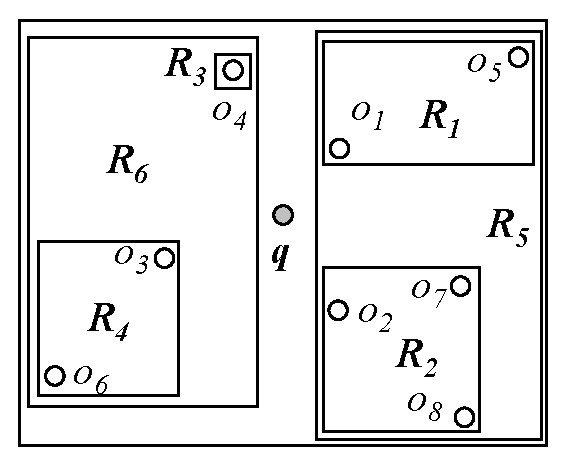
\includegraphics[scale=0.4]{figure/figures1}
    \end{tabular}
    &
    \begin{tabular}{|c|c|}
    \hline
    object & words \\ \hline \hline
    $o_1$ & $t_1, t_2$ \\
    $o_2$ & $t_2, t_3$ \\
    $o_3$ & $t_1, t_3$  \\
    $o_4$ & $t_1, t_5$ \\
    $o_5$ & $t_2, t_4$ \\
    $o_6$ & $t_4, t_6$ \\
    $o_7$ & $t_4, t_5$ \\
    $o_8$ & $t_1, t_5$ \\
    \hline
    \end{tabular}
    \\
    (a) object locations & (b) object descriptions
 \end{tabular}
\vspace{-6pt} \caption{A Dataset of Spatial Keyword Objects}
\label{fig:map} \vspace{-6pt}
\end{figure}

\begin{figure}[!hbt]
\vspace{-5pt} \centering
 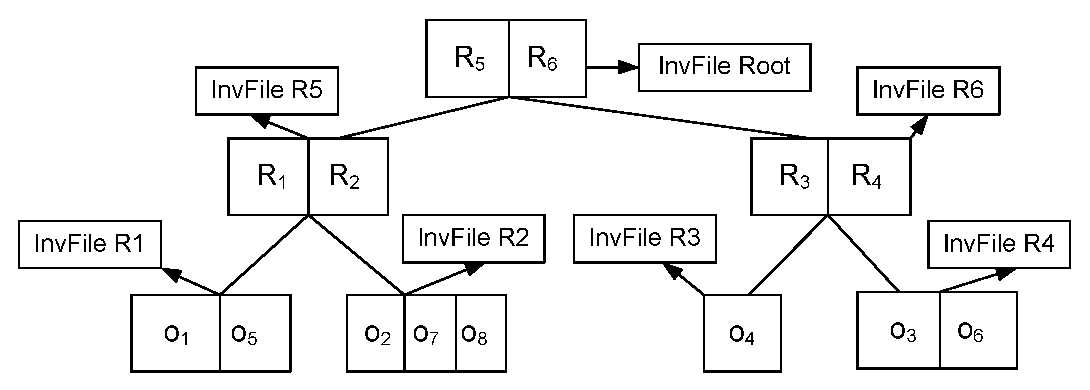
\includegraphics[scale=0.4]{figure/irtree}
\vspace{-8pt} \caption{Example IR-Tree} \label{fig:IRtree}
\vspace{-9pt}
\end{figure}

\begin{table}[!hbt]
  \centering \small
\vspace{-2pt}
  \caption{Content of Inverted Files of the IR-Tree}\label{table:InvertedList}
  \begin{tabular}{|@{ }l@{ }|@{ }l@{ }|@{ }l@{ }|@{ }l@{ }|@{ }l@{ }|@{ }l@{ }|@{ }l@{ }|}
    \hline
    %$\mathit{InvF}$-$\mathit{root}$ & $\mathit{InvF}$-$R_5$ & $\mathit{InvF}$-$R_6$ & $\mathit{InvF}$-$R_1$         & $\mathit{InvF}$-$R_2$ & %$\mathit{InvF}$-$R_3$ & $\mathit{InvF}$-$R_4$\\
    $\mathit{Root}$ & $R_5$ & $R_6$ & $R_1$  & $R_2$ & $R_3$ & $R_4$\\
    \hline \hline
    $t_1$: $R_{5},R_{6}$    & $t_1$: $R_{1},R_{2}$  & $t_1$: $R_{3}, R_{4}$ & $t_1$: $o_{1}$     & $t_1$: $o_{8}$  & $t_1$: $o_{4}$ & $t_1$: $o_{3}$\\
    $t_2$: $R_{5}$    & $t_2$: $R_{1},R_{2}$ & $t_3$: $R_{4}$ & $t_2$: $o_{1},o_{5}$       & $t_2$: $o_{2}$        & $t_5$: $o_{4}$ & $t_3$: $o_{3}$\\
    $t_3$: $R_{5},R_{6}$    & $t_3$: $R_{2}$       & $t_4$: $R_{4}$ & $t_4$: $o_{5}$       & $t_3$: $o_{2}$        &                & $t_4$: $o_{6}$\\
    $t_4$: $R_{5},R_{6}$    & $t_4$: $R_{1},R_{2}$ & $t_5$: $R_{3}$ &                      & $t_4$: $o_{7}$        &                & $t_6$: $o_{6}$\\
    $t_5$: $R_{5},R_{6}$    & $t_5$: $R_{2}$       & $t_6$: $R_{4}$ &                      & $t_5$: $o_{7},o_{8}$  &                &\\
    $t_6$: $R_{6}$          &              &            &                      &                       &                &\\
    \hline
  \end{tabular}
  \vspace{-3pt}
\end{table}



\subsection{Approximation Algorithm}

We show that the first subproblem is NP-complete by a reduction
from the Weighted Set Cover (WSC) problem in Lemma~\ref{lemma:nphard1}.
The reduction in the proof is approximation preserving. Thus, the
approximation properties of the WSC problem carry over to our problem.

For the WSC problem, it is known (see~\cite{setcover}) that a greedy
algorithm is an $H_k$-approximation algorithm for the weighted
$k$-set cover, where $H_k$ = $\sum_{i =1}^{k} \frac{1}{i}$ is the
$k$-th harmonic number. In our problem, $k$ is the number of query
keywords.
%
Thus, we can adapt the greedy algorithm to process the \textsc{TYPE1}
spatial group keyword query.

A straightforward method of adapting the greedy algorithm is to
decompose the given user query $q$ dynamically into a
sequence of partial queries, each containing a different set of
keywords depending on the preceding partial queries, and then to
evaluate these partial queries.
%
Specifically, we start with the user query $q$, which can be regarded
as the first partial query, and we find the object with the lowest
cost that covers part or all of the keywords in $q$. The object is
added to the result set. The uncovered keywords in $q$ form a new
partial query with the same spatial location as $q$.  We then
find an object with the lowest cost that covers
part or all of the keywords in the new partial query. This process
continues until all keywords are covered or some keyword cannot be
covered by any object. This method needs to scan the dataset multiple
times, once for each partial query.

%A straightforward method of adapting the greedy algorithm is to
%1)~check all the objects to find the object that contain keywords in
%query $q$ and has the lowest cost, 2)~remove the keywords in the
%object from $q.\psi$, and then repeat step 1) until all keywords in
%$q$ are covered. This method needs to scan the data multiple times.
%
%To avoid multiple scans, we propose a greedy algorithm on top of the
%IR-tree.
%%
%The idea is to dynamically decompose the given user query $q$ into a
%sequence of partial queries, each containing a different set of
%keywords depending on the preceding partial queries, and then to
%evaluate these partial queries.
%%
%Specifically, we start with the user query $q$, which can be regarded
%as the first partial query, and we find the object with the lowest
%cost that covers part or all of the keywords in $q$. The object is
%added to the result set. The uncovered keywords in $q$ form a new
%partial query with the same spatial location as $q$.  We process the
%new partial query to find an object with the lowest cost that covers
%part or all of the keywords in the partial query. This process
%continues until all keywords are covered or some keyword cannot be
%covered by any object.

To avoid multiple scans, we propose a greedy algorithm on top of the IR-tree.
We proceed to focus on two aspects of the idea that are important to
the performance: (1) how to find the object with the lowest cost for
each partial query using the IR-tree, and (2) whether we can reuse the computation for
the preceding partial query when computing the next partial query.

Given a partial query $q_s$, we adopt the best-first strategy to
traverse the IR-tree. We use a min-priority queue to maintain the
intermediate results. The key of the queue is the cost of each
element. The cost of an object $o$ is computed by $\frac{\Dist(q,
  o)}{|o.\psi \cap q_s.\psi|}$; the cost of a node entry $e$ is
computed by $\frac{\minDist(q, e)}{|e.\psi \cap q_s.\psi|}$, where
\minDist$(q, e)$ represents the minimum distance between $q$ and $e$.

\begin{lemma}\label{lemma:greedy1}
  Given a partial query $q_s$ and an IR-tree, the cost of a node is
  a lower bound of the cost of any of its child nodes.

  \proof Given a node $e$ and any of its child nodes $e'$, we have
  \minDist$(q, e)$ $\leq$ \minDist$(q, e')$, and $|e.\psi \cap
  q_s.\psi| \geq |e'.\psi \cap q_s.\psi|$.
\end{lemma}

Lemma~\ref{lemma:greedy1} says that the cost of a node is a lower
bound of the costs of all objects in the subtree rooted at the node.
Thus, if the cost exceeds that of some object that has been visited,
we can disregard all objects in the subtree for $q_s$. This
guarantees the correctness of the best-first strategy for finding an
object with the lowest cost for a partial query $q_s$.

We next discuss whether we can reuse the computation for preceding
partial queries. An obvious method is to process each partial query
from scratch. However, this incurs repeated computation when
a node or an object is visited for multiple times. To avoid this, we divide the entries
(corresponding to leaf and non-leaf nodes) in the priority queue
into two parts: (1) the entries that have already been visited when
processing previous partial queries, and (2) the entries that have not
yet been visited.

\begin{lemma}\label{lemma:greedy2}
  The elements in the priority queue that have been visited when
  processing previous partial queries can be disregarded when
  processing a new partial query.

  \proof The keyword set of a previous partial query is a superset of
  the keyword set of a new partial query. For a visited node, all its
  entries containing keywords of the new partial query have been
  enqueued into the priority queue; thus, we can disregard the
  elements that have been visited.
\end{lemma}

The pseudocode is outlined in Algorithm~\ref{alg:greedyindex}. The
algorithm uses a min-priority queue for the best-first search with the
cost as the key.
%
Variable $mSet$ keeps the keyword set of the current partial query,
and $pSet$ keeps the keyword set of the preceding partial query.
%
For each partial query, we use the best-first search to find an object
that overlaps with the query keyword $mSet$ and has the lowest cost.
%
The algorithm computes the cost for a non-object node (line~23) and the
cost for an object (line~25).

Whenever the algorithm pops an object from $U$, it is guaranteed
that the text description of the object overlaps with $mSet$ (the
keyword set of the current partial query), and that the object has
the lowest cost. Thus, it becomes part of the result.
%
The algorithm proceeds with the next partial query by changing the
keyword component (line~12). Based on Lemma~\ref{lemma:greedy2}, we do
not need to scan all objects to process the new partial query.
%
Rather, we only have to update the unvisited elements in the priority
queue with the new cost based on the new partial query
(lines~13--16). We then use the best-first search to process the new
partial query.

\begin{algorithm}[!t]\label{alg:greedyindex} \small
\caption{Type1Greedy( $q$, $irTree$)}\label{alg:subquery}

    $U$ $\leftarrow$ new min-priority queue\;
    %
    $U$.$\mathsf{Enqueue}$($irTree.root,0$)\; $V \leftarrow \emptyset$; $Cost \leftarrow $ 0\;
    %
    $mSet \leftarrow q.\psi$; $pSet \leftarrow q.\psi$\;

    \While{ $mSet \neq \emptyset$ }
    {

        \While{$U$ is {\bf not} empty}
        {
            $e \leftarrow U.$$\mathsf{Dequeue}$()\;

            $Cost \leftarrow Cost + e.Key$\;

            \If{$\mathit{e}$ is an object}
            {
                $V$ $\leftarrow$ $V$ $\cup$ $e$\;
                $pSet$ $\leftarrow$ $mSet$ \;
                $mSet$ $\leftarrow$ $mSet \setminus e.\psi$\;
                %adjust priority queue
                \For{each entry $e'$ in $U$}
                {
                    %\lIf {$e.\lambda \cap$ $mSet$ $\neq \emptyset$}
                    \If {$e'.\lambda \cap$ $e.\lambda$ $\neq \emptyset$}
                    {
                        $e'$.key = $\frac{e'.key * |e'.\lambda \cap mSet|}{|e'.\lambda \cap pSet|} $ \;
                    }
                    \lElse {remove $e$ from $U$\;}
                }
                reorganize priority queue $U$ using new key values\;
                break\;
            }
            \Else
            {
                read the posting lists of $\mathit{e}$ for keywords in $mSet$\;
                \For{each entry $e'$ in node $\mathit{e}$}
                {
                    \If {$mSet \cap e'.\psi \neq \emptyset$} %{\bf and}
                    {
                        \If{$\mathit{e}$ is a non-leaf node}
                        {
                            $U$.$\mathsf{Enqueue}$($e'$, $\frac{\minDist(q,e')}{|mSet\cap e'.\psi|}$ );
                        }
                        \Else
                        {
                            $U$.$\mathsf{Enqueue}$($e'$, $\frac{\Dist(q,o)}{|mSet\cap o.\psi|} $);
                        }
                    }
                }
            }
        }
    }

    {\bf return} $Cost$ and $ V $ \tcp*[r]{ results}\vspace{-1ex}
\end{algorithm}


\subsection{Exact Algorithm}

The number of keywords of a query may be small in some
applications. This motivates us to develop an exact algorithm for
processing the TYPE1 spatial keyword group query.

We present a dynamic programming algorithm that does not use an
index in Section~\ref{sec:sub:noindex}, and we present a version of
the algorithm that uses an index to prune the search space in
Section~\ref{sec:type1:index}.


\subsubsection{Exact Algorithm Without an Index}
\label{sec:sub:noindex}

An obvious exact algorithm enumerates every subset of spatial objects
whose text descriptions overlap with the query keyword set
in $D$.For each such subset, the algorithm then checks whether
the subset covers all query keywords and computes its
cost. This yields an exponential running time in terms of the number
of objects, which is very expensive if $D$ is large.

A better method is to perform the exhaustive search on a
smaller set of objects. We proceed to introduce a lemma that lays
the foundation for the algorithm to be proposed.

\begin{lemma} \label{lemma:bestobj} Consider a query $q$ and two
  objects $o_i$ and $o_j$, each of which contains a subset of the query
  keywords. Let $ws_i = q.\psi \cap o_i.\psi$ and $ws_j = q.\psi
  \cap o_j.\psi$. If $\Dist(q, o_i) < \Dist(q, o_j)$, \{$o_i$\}
  is a better group than \{$o_j$\} for any keyword subset of
  $ws_i \cap ws_j$ .

  \proof Obvious since $o_i$ always incurs lower cost than does $o_j$ for
  any keyword subset $ws_i \cap ws_j$.
\end{lemma}

According to the lemma, given a subset of query keywords $ws$, among the
objects covering $ws$, the one that is the closest to the query
contributes the lowest cost to $ws$.

\begin{example} \label{ex:lemma33}
  Consider a query $q$ with keywords $q.\psi$ = \{$t_1, t_2, t_3$\} and
  the four objects in Table~\ref{tbl:example}.
%
  We know that $\Dist(q, o_1)< \Dist(q, \\o_2)$ and $o_1 \cap o_2$ =
  \{$t_2$\}. According to lemma~\ref{lemma:bestobj}, \{$o_1$\} is
  a better result set for the query with keyword set \{$t_2$\}.
\end{example}

\begin{table}[h]\vspace{-2ex}
  \centering \small
  \begin{tabular}{|c|c|c|c|c|}
    \hline
    &   $o_1$ & $o_2$ & $o_3$ & $o_4$ \\
    \hline
    Distance to the query & 1 & 2 & 2.5 & 4\\
    \hline
    Keywords & $t_1$,$t_2$ & $t_2$,$t_3$ & $t_1$,$t_3$ & $t_1$\\
    \hline
  \end{tabular}\vspace{-1ex}\caption{Example data set}\label{tbl:example}\vspace{-2ex}
\end{table}

Since the set of query keywords is small, the number of its subsets
is not large although it is exponential to the number of query
keywords. For each subset of query keywords, we  find the object
that covers the subset of query keywords and has the lowest costs
according to Lemma~\ref{lemma:bestobj}. Then an exhaustive search on
these objects can find the best group. However, this method is
time-consuming since it runs exponentially in terms of the number of
objects, which can be exponential in the number of query keywords.


%Suppose there are $n$ keywords
%in the query text component, only at most $(2^n-1)$ objects need to be
%considered. Although this method outperforms the first method a lot, it is still
%quite time consuming since its time complexity is O($2^{(2^n-1)}$).

Instead, we develop a dynamic programming algorithm with
exponential running time in terms of the number of query keywords.
The idea of the algorithm is summarized as follows:~Given a query $q$
with $n$ ($= |q.\psi|$) keywords, we process the subsets of $q.\psi$
in breadth-first order, i.e., we process subsets in ascending order
of their length. For each subset $X$ of $q.\psi$, we find the best
set of covering objects, i.e., a set of objects that cover
$X$ and have the lowest cost, by utilizing the best
covering sets of the subsets of $X$.

Existing WSC algorithms are mostly approximation algorithms. Several
recent proposals~\cite{exp1,exp2} have good (e.g., constant)
approximation guarantees with moderately exponential running time.
%We are not aware of published work on exact WSC algorithms.
%
Bj\"{o}rklund et al.~\cite{exp3} propose an exact algorithm for the
unweighted set cover problem using the inclusion-exclusion principle,
which is not directly applicable to the WSC problem.

Formally, let $F$ be the set of all subsets of $q.\psi$.  For each
subset $X \subseteq q.\psi$, we denote the set of objects that cover
$X$ and has the lowest cost by \Group$(X)$ and the cost of covering
set $X$ by \Cost$(X)$.

Our dynamic programming algorithm avoids enumerating all the set
partitions. Equation~\ref{eq:cost} shows the approach to computing
the lowest cost for each subset $X$. If $X$ is
not covered by any object $o$, its cost is initialized to
$\infty$; otherwise, its cost is initialized to the cost of the best covering
object, as shown in Equation~\ref{eq:cost}. Then the
dynamic programming idea is adopted to find the lowest cost of each
subset $X$ in ascending order of the length of $X$. Specifically,
for each $X$, we check each pair of component subsets (whose optimal
costs are already known) to find a pair with the lowest cost. Note
that the optimal set of two subsets may share some objects whose
costs are computed by $\mathsf{oCost}$.

\vspace{-2ex}
\begin{equation}\vspace{-0.5ex} \small \label{eq:cost}
\Cost(X) = \left\{
            \begin{array}{ll}
               \min_{o \in D \wedge X
\subseteq o.\psi} \{\Dist(q, o) \}, & \exists o (X \subseteq o.\psi) \\
                   \infty, & \mathrm{otherwise}
              \end{array}
       \right.
\end{equation}
\begin{equation*}
\small
\Cost(X) =     \min_{S \in F \wedge S \subseteq X} \{\Cost(X
\setminus S) + \Cost(S) - \mathsf{oCost}(S, X \setminus S)
\}  \\
\end{equation*} \vspace{-1ex}
\begin{equation}\label{eq:ocost}
\small
\mathsf{oCost}(S, X \setminus S) = \sum_{o \in \Group(X \setminus S)
\cap \Group(S)}
\Dist(o,q)\\
\end{equation}

\begin{equation}\label{eq:group}
\small
\begin{aligned}
\mathsf{Group}(X) &=
\begin{cases}
\arg\min_{o \in D \wedge X \subseteq o.\psi} \{\Dist(q, o)
\}, & \exists o (X \subseteq o.\psi) \\
\emptyset, & \mathrm{otherwise}
\end{cases}\\
%
S* = &\mathop{\arg\min}_{S \in F \wedge S \subseteq X} \{\Cost(X
\setminus S) + \Cost(S) - \mathsf{oCost}(S, X \setminus S) \}
\\\vspace{-4ex}
\ \ \ &\mathsf{Group}(X) = \mathsf{Group}(S*) \cup
\mathsf{Group}(X \setminus S*)
\end{aligned}
\end{equation}

To implement the algorithm efficiently, we encode the subsets.  A
query $q$ with $n$ keywords $q.\psi = \{t_1, t_2, \ldots, t_n\}$ has
$(2^n-1)$ non-empty subsets of keywords. We encode each subset $X$ by
an integer $i$ of $n$ bits, where each bit corresponds to a keyword in
$q$.
%
If the $j^{th}$ keyword is contained in $X$, the $j^{th}$ bit
in the binary format of $i$ is set to 1; otherwise, it is set to 0.
%
For example, for $q.\psi$=\{$t_1, t_2, t_3$\}, we can encode subset
\{$t_1$\} by 1, \{$t_2$\} by 2, and \{$t_1, t_2$\} by 3.

We maintain two arrays: $\Cost[i]$ records the lowest cost of the
subset that is encoded by integer $i$, and $\Group[i]$ records the
group of objects that contribute to the lowest cost.
Equations~\ref{eq:ocost} and~\ref{eq:group} can be rewritten as the
following equation:
%
\begin{equation}\small
\begin{aligned}
\Cost[i] &= \min_{j, i\&j = j} \{ \Cost[j] + \Cost[i-j]- \mathsf{oCost}(i, j)\}\\
\mathsf{oCost}(i, j) &= \sum_{o \in \Group[i] \cap \Group[i-j]} \Dist(o,q)\\ %\|i\&j == j \}\\
opt &= \mathop{\arg\min}_{j, i\&j = j} \{ \Cost[j] + \Cost[i-j]- \mathsf{oCost}(i, j)\} \\%Cost[i]\\
\Group[i] &= \Group[opt] \cup \Group[i-opt]
\end{aligned} \label{eq:iter}
\end{equation}
%
Here, $\&$ is the bit-wise AND operator, and $i\&j$ = $j$ states that
the set represented by $j$ is a subset of the set represented by
$i$.

\begin{algorithm}[!t] \small
\caption{\label{alg:pb1base} \bf {Type1ExactNoIndex} $(q, D)$}

%\KwIn{ A query $q=\langle \lambda, \psi\rangle$, Dataset $D$}

%\KwOut{The best group of objects and the lowest cost}

$n$ $\leftarrow$  $|q.\psi|$\;

\lFor{$i$ from $1$ to $2^n-1$}
{
\Cost$[i]$ $\leftarrow$ $\infty$, \Group$[i]$ $\leftarrow$
$\emptyset$\;
}


\For {each object $o_i$ in $D$} {
    %$ks$ $\leftarrow$ $o_i.\psi \bigcap q.\psi$\;
    \If{$o_i.\psi \cap q.\psi \neq \emptyset$ }
    {
        Dist[$o_i$] $\leftarrow$ \Dist($o_i, q$)\;
        \For {each subset $s_i$ in $o_i.\psi \cap q.\psi$}
        {
            i $\leftarrow$ $\mathsf{MapToInteger}$($s_i$)\;
            \If{ \Cost$[i]$ $>$ \Dist$[o_i]$}
            {
                \Cost[$i$] $\leftarrow$ \Dist$[o_i]$\;
                \Group[$i$] $\leftarrow$ \{$o_i$\}\;
            }
        }
    }
}

\For{$i$ from $1$ to $2^n-1$} {
    $minValue$ $\leftarrow \infty$,     $bestSplit$ $\leftarrow$ 0\;
    \For{$j$ from $1$ to $i/2$}
    {
        \If{$j$ $\&$ $i$ = $j$}
        {
            $S$ $\leftarrow$ \Group[$j$] $\bigcap$ \Group[$i-j$]\;
            $oDist$ $\leftarrow$ 0\;
            \For{each object $o$ in $S$}
            {
               $oDist$ $\leftarrow$ $oDist$ + \Dist[$o$]\;
            }
            $cost$ $\leftarrow$ \Cost[$j$] + \Cost[$i-j$] $-$ $oDist$\;
            \If{$cost < minValue$}
            {
                $minValue \leftarrow cost$\;
                $bestSplit \leftarrow j$\;
            }
        }
    }
    \If{\Cost$[i]$ $>$ $minValue$ }
    {
        \Cost[$i$] $\leftarrow$ $minValue$\;
        \Group[$i$] $\leftarrow$ \Group[$bestSplit$] $\cup$ \Group[$i- bestSplit$]\;
    }
} \Return \Cost[$2^n-1$] and \Group[$2^n-1$]\vspace{-1ex}

\end{algorithm}

The pseudocode is outlined in Algorithm~\ref{alg:pb1base}. We
progressively compute $\Cost[i]$ and $\Group[i]$ from $i=1$ to $(2^n-1)$.
When $i$ = $(2^n-1)$, we get the results with the lowest cost,
$\Cost[2^n-1]$, and the best group, $\Group[2^n-1]$.
%
We scan the dataset $D$. For each single object that overlaps
with query keyword set $q.\psi$, we check whether the object contributes to
the lowest cost for a keyword subset (lines~3--10).
%
If a keyword subset is not contained by any single object, its cost
is initialized to $\infty$.

The algorithm proceeds to use Equation~\ref{eq:iter} to compute
the lowest cost for each subset (lines~11--25). We check each
subset, represented by $j$, of the current keyword subset,
represented by $i$, to see whether the subset represented by $j$ and
the subset represented by $(i -j)$ contribute a lower cost
(lines~13--22). The lowest cost from combining two subsets is kept
in $minValue$, and the integer that represents the corresponding subset
is kept in $bestSplit$.
%
If the $minValue$ contributed by aggregating two subsets is smaller
than the current lowest cost of the keyword subset represented by $i$,
we update its cost $\Cost[i]$ and update the group of objects
$\Group[i]$ that covers it (lines~23--25). Finally, we return the
lowest cost and the best group (line~26).


The algorithm scans the whole dataset $D$ in lines~3--10, and it
finds the best group according to Equation~\ref{eq:iter} in lines~11--22.
Therefore, it runs exponentially in terms of the number of query keywords
and linearly in terms of the size of the dataset.


\begin{example}
  We proceed to illustrate Algorithm~\ref{alg:pb1base}. Given a query
  $q$ with the keywords set $q.\psi$ = \{$t_1, t_2, t_3$\} and three objects
  $o_1$, $o_2$, and $o_3$ with description:
  $o_1.\psi$ = \{$t_1, t_2$\} and \Dist$(q, o_1)$ = 1; $o_2.\psi$
  =\{$t_2, t_3$\} and \Dist$(q, o_2)$ = 2; $o_3.\psi$ = \{$t_1,
  t_2, t_3$\} and \Dist$(q, o_3)$ = 4. Lines~3--10 return the
  following results:

\begin{table}[h]\vspace{-2ex}
  \centering \small
  \begin{tabular}{|c|c|c|c|c|c|c|c|}
    \hline
    $i$    & 1 & 2 & 3 & 4 & 5 & 6 & 7\\
    \hline
    Cost & 1 & 1 & 1 & 2 & 4 & 2 & 4\\
    \hline
    Group & $o_1$ & $o_1$ & $o_1$ & $o_2$ & $o_3$ & $o_2$ & $o_3$\\
    \hline
  \end{tabular}\vspace{-2ex}
\end{table}

We subsequently utilize these values to compute the final results. For
example, when computing \Cost[5], we determine that \{$o_1,
o_2$\}(\Cost[1]+\Cost[4]) is better than \{$o_3$\}, and we update its
value. Finally, we have the following results:

\begin{table}[h]\vspace{-2ex}
  \centering \small
  \begin{tabular}{|c|c|c|c|c|c|c|c|}
    \hline
    $i$    & 1 & 2 & 3 & 4 & 5 & 6 & 7\\
    \hline
    Cost & 1 & 1 & 1 & 2 & 3 & 2 & 3\\
    \hline
    Group & $o_1$ & $o_1$ & $o_1$ & $o_2$ & $o_1, o_2$ & $o_2$ & $o_1, o_2$\\
    \hline
  \end{tabular}\vspace{-2ex}
\end{table}\vspace{-2ex}
\end{example}


\subsubsection{Exact Algorithm Using an Index}\label{sec:type1:index}

The dynamic programming algorithm presented above needs to scan the
whole dataset. This has two drawbacks: (1)~it wastes computation
when checking many unnecessary objects that do not contain any query
keyword, and (2)~all the objects whose text descriptions overlap
with the query keywords are scanned to obtain the lowest costs for
the query keyword subsets.

To overcome the first drawback, we utilize the
IR-tree that enables us to retrieve only the objects that contain some
query keywords while avoiding checking the objects containing no query
keywords.
%
For the second drawback, we show that it is not always necessary to
scan all the objects covering part of the query keywords.
%%
%We proceed
%to introduce several lemmas that will lay the foundation for the
%algorithm to be proposed.
%
%
%\begin{lemma} \label{lemma:bestobj} Consider a query $q$ and two
%  objects $o_i$ and $o_j$ that contain a subset of the query
%  keywords. Let $ws_i = q.\psi \cap o_i.\psi$ and $ws_j = q.\psi
%  \cap o_j.\psi$. If $\Dist(q, o_i) < \Dist(q, o_j)$, {$o_i$}
%  is a better group than {$o_j$} for any keyword subset of
%  $ws_i \cap ws_j$ .
%
%  \proof Obvious since $o_i$ always incurs lower cost than does $o_j$ for
%  any keyword subset $ws_i \cap ws_j$.
%\end{lemma}
%
%According to the lemma, given a subset of query keywords $ws$, among the
%objects covering $ws$, the one that is the closest to the query
%contributes the lowest cost to $ws$.
%
%\begin{table}[h]\vspace{-2ex}
%  \centering \small
%  \begin{tabular}{|c|c|c|c|c|}
%    \hline
%    &   $o_1$ & $o_2$ & $o_3$ & $o_4$ \\
%    \hline
%    Distance to query & 1 & 2 & 2.5 & 4\\
%    \hline
%    Keywords & $t_1$,$t_2$ & $t_2$,$t_3$ & $t_1$,$t_3$ & $t_1$\\
%    \hline
%  \end{tabular}\vspace{-2ex}\caption{Example data set}\label{tbl:example}\vspace{-4ex}
%\end{table}
%
%\begin{example} \label{ex:lemma33}
%  Consider a query with keywords $q.\psi$ = \{$t_1, t_2, t_3$\} and
%  the four objects in Table~\ref{tbl:example}.
%%
%  We know that $\Dist(q, o_1)< \Dist(q, o_2)$ and $o_1 \cap o_2$ =
%  \{$t_2$\}. According to lemma~\ref{lemma:bestobj}, {$o_1$} is
%  a better result set for the query with keyword set \{$t_2$\}.
%\end{example}

We propose the following principle for our algorithm: we process
objects in ascending order of their distances to a query $q$. By
following that order, we know that the lowest cost of a subset is
always contributed by a single or a group of closer objects based on
Lemma~\ref{lemma:bestobj}.

\begin{lemma}\label{lemma:subset_costs}
  Consider a query $q$. If we process objects in ascending order of
  their distances to $q$, when we reach an object $o_i$ containing
  a query keyword subset $ws$, all subsets of $ws$ will get their lowest costs.

  \proof Obvious since all objects to be visited after $o_i$ have
  larger cost for any subset of $ws$; thus, its lowest cost is either
  contributed by $o_i$ or by objects visited earlier.
\end{lemma}

\begin{example}
  Recall the query in Example~\ref{ex:lemma33}. We first process
  object $o_1$, and we know 1 is the lowest costs of subsets \{$t_1, t_2$\},
  \{$t_1$\}, and \{$t_2$\}.
%
  Then we reach $o_2$, and we know 2 is the lowest costs of subsets \{$t_2,
  t_3$\} and \{$t_3$\} (\{$t_2$\} already has lowest cost 1).
\end{example}


Based on Lemma~\ref{lemma:subset_costs}, we can derive a stopping
condition for our algorithm---we reach an object that contains all
the query keywords. However, if no such object exists in the
dataset, the algorithm is still required to scan to the furthest
object containing some query keywords before it can stop. In the
example in Table~\ref{tbl:example}, we need to read all the
four objects. But if the third furthest object $o_3$ covers \{$t_1,
t_2, t_3$\}, we need not read $o_4$.

We proceed to present an additional stopping condition.

\begin{lemma}\label{lemma:upper}
Given two query keyword subsets $ws_i$ and $ws_j$, and with union
$ws_u = ws_i \cup ws_j$, we have \Cost$(ws_u)$ $\leq$
\Cost$(ws_i)$ + \Cost$(ws_j)$.

\proof Obvious from Equations~\ref{eq:cost}--\ref{eq:group}.
\end{lemma}

Based on Lemma~\ref{lemma:upper}, for any two keyword subsets whose lowest
costs are known, we can obtain an upper bound of the lowest cost
value for the keyword subset that is the union of the two keyword subsets.
We denote the upper bound by $Cost_u$.

In our algorithm, we keep track of the upper bounds for the
subsets whose costs are still unknown. Whenever we reach an object
from which some keyword subset gets its lowest cost (according to
Lemma~\ref{lemma:subset_costs}), the subset, together with each of
the subsets that have either lowest costs or upper bounds of cost
(i.e., the keyword subsets that are covered by visited objects), are
used to update the upper bound cost values of the corresponding
union keyword subsets.

\begin{example}
Recall Example~\ref{ex:lemma33}. After the object $o_2$ is scanned,
\{$t_3$\} gets its lowest cost 2. We can compute an upper bound
for \{$t_1, t_3$\} using the costs of \{$t_1$\} and \{$t_3$\}, i.e.,
$Cost_u(\{t_1, t_3\})$ = \Cost(\{$t_1$\})+\Cost(\{$t_3$\}) = 3
(covered by $o_1$ and $o_2$). Similarly, we can also compute an upper
bound value 3 for \{$t_1, t_2, t_3$\} using the costs of \{$t_1, t_2$\} and
\{$t_3$\}, and the set is also covered by $o_1$ and $o_2$.

When we reach $o_3$, we get a lower cost of 2.5 for \{$t_1,
t_3$\}(the previous upper bound of 3 is updated). Then \{$t_1, t_3$\} are
 combined with \{$t_2$\} to form \{$t_1, t_2, t_3$\} with a cost of
3.5. Since this value exceeds its current upper bound, no
update is needed.
\end{example}

We are ready to introduce a lemma that provides an early stopping
condition for our algorithm.

\begin{lemma}\label{lemma:cost_update}
Suppose that we scan objects in ascending order of their distances
to $q$. Given a keyword subset $ws$, when we reach object $o_i$, and if
$\Dist(q, o_i) \geq Cost_{u}(ws)$, then $\Cost(ws) = Cost_{u}(ws)$,
where $Cost_{u}(ws)$ is the current upper bound of $ws$.

\begin{proof}
We prove this by contradiction.
If any object $o_j$ further to $q$ than $o_i$ is a member of the best
group then it must have
\begin{displaymath}
\Cost(ws) \geq \Dist(q, o_j) \geq \Dist(q, o_i) \geq Cost_{u}(ws)
\end{displaymath}
Since $Cost_{u}(ws)$ cannot be smaller than $\Cost(ws)$, no further
object will be contained in the best group. In addition,
$Cost_{u}(ws)$ is the current minimum cost value, and thus it
becomes the lowest cost of $ws$.
\end{proof}\vspace{-2ex}
\end{lemma}

\begin{example}
Recall again Example~\ref{ex:lemma33}. By following ascending order of
distances, when the algorithm reaches $o_4$ (\Dist$(q, o_4)$ = 4), we
can conclude that $Cost_u(\{t_1, t_2, t_3\})$ = 3 is the lowest cost
and that the best group is ($o_1$, $o_2$).
\end{example}


\begin{algorithm}[!h]
\small \caption{Type1ExactWIndex($q$, $irTree$)}\label{alg:pb1tree}
%\KwIn{A query $q=\langle \lambda, \psi\rangle$ and IR-Tree index $irTree$.}

%\KwOut{The best group of objects and the lowest cost}

$markedSet$ $\leftarrow \emptyset$, $valuedSet$ $\leftarrow
\emptyset$\;

$n$ $\leftarrow$ $|q.\psi|$\;

\lFor{$i$ from $1$ to $2^n-1$} { \Cost$[i]$ $\leftarrow$ $\infty$,
\Group$[i]$ $\leftarrow$ $\emptyset$\; }

$U$ $\leftarrow$ new min-priority queue\;
%
$U$.$\mathsf{Enqueue}$($irTree.root,0$)\;

%
    \While{$U$ is {\bf not} empty}
    {
        $e \leftarrow U.$$\mathsf{Dequeue}$()\;

        $ks$ $\leftarrow$ $q.\psi \bigcap \mathit{e}.\psi$ \;

        \If{$ks$ $\not\in$ $markedSet$}
        {
            \If{$\mathit{e}$ is a non-leaf node}
            {
                \ForEach{ entry $e'$ in node $\mathit{e}$}
                {

                    \lIf {$q.\psi \bigcap e'.\psi$$ \neq \emptyset$ and $q.\psi \bigcap e'.\psi$ $\not\in markedSet$}
                    {
                       $U$.$\mathsf{Enqueue}$($e'$, $\minDist(q,e')$);
                    }
                }
            }
            \ElseIf{$\mathit{e}$ is a leaf node}
            {
                \ForEach{ object $o$ in leaf node $\mathit{e}$}
                {
                    \lIf {$q.\psi \bigcap o.\psi \neq \emptyset$ and $q.\psi \bigcap \mathit{o}.\psi \not\in markedSet$}
                    {
                        $U$.$\mathsf{Enqueue}$($o$, $\Dist(q,o)$);
                    }
                }
            }
            \Else(\tcp*[f]{$\mathit{e}$ is an object})
            {
                \ForEach{set $S$ $\in$ $valuedSet$}
                {
                    $i$ $\leftarrow$ $\mathsf{MapToInteger}$($S$)\;
                    \If{\Cost$[i]$ $<$ \Dist($q, e$)}
                    {
                        \If(\tcp*[f]{Lemma~\ref{lemma:cost_update}}){i = $2^n\!-\!1$}
                        {\Return \Cost[$2^n\!-\!1$] and \Group[$2^n-1$]\;}
                        $valuedSet$ $\leftarrow$ $valuedSet$ $\backslash$ $S$\;
                        $markedSet$ $\leftarrow$ $markedSet$ $\bigcup$ $S$\;
                    }
                }
                $tempSet$ $\leftarrow \emptyset$\;
                \ForEach (\tcp*[h]{Lemma~\ref{lemma:subset_costs}}){subset $ss$ $\subseteq$ $ks$}
                {
                    \If{$ss$ $\not\in$ $markedSet$}
                    {
                        $i$ $\leftarrow$ $\mathsf{MapToInteger}$($ss$)\;
                        $markedSet$ $\leftarrow$ $markedSet$ $\bigcup$ $ss$\;
                        $tempSet$ $\leftarrow$ $tempSet$ $\bigcup$ $ss$\;
                        \If{$ss$ $\in$ $valuedSet$}
                        {
                            $valuedSet$ $\leftarrow$ $valuedSet$ $\backslash$ $ss$\;
                        }
                        \Cost[$i$] $\leftarrow$ \Dist($e, q$)\;
                        \Group[$i$] $\leftarrow$ \{$\mathit{e}$\}\;
                            %\tcp{\scriptsize\!\!\!stop \!condition\! derived\! from \!Lemma~\ref{lemma:subset_costs}}
                        \If(\tcp*[f]{Lemma~\ref{lemma:subset_costs}}){$j$ = $2^n-1$}
                        {\Return \Cost[$2^n-1$] and \Group[$2^n-1$]\;}
                    }
                }
                \ForEach{ set $ts \in tempSet$}
                {
                    $j$ $\leftarrow$ $\mathsf{MapToInteger}$($ts$)\;
                    \For{$i$ from $1$ to $2^n-1$}
                    {
                        \lIf{\Cost$[i]$ $= \infty $ } { continue}\;
                        $unionKey$ $\leftarrow$ $i | j$\;
                        \If{$unionKey$ = $i$ $\wedge$ unionKey = $j$}
                        {\bf continue;}
                        $D$ $\leftarrow$ \Cost[$i$] + \Dist($e, q$)\;
                        \If{\Cost$[$unionKey$]$ $>$ D }
                        {
                            \Cost[$unionKey$] $\leftarrow$ $D$\;
                            \Group[$unionKey$] $\leftarrow$ \Group[$i$] $\bigcap$ \{$\mathit{e}$\}\;
                        }
                    }
                }
            }
        }
    }
\Return \Cost[$2^n-1$] and \Group[$2^n-1$]\;\vspace{-1ex}
\end{algorithm}\vspace{-1ex}

The pseudocode is described in Algorithm \ref{alg:pb1tree}.
%
All the keyword subsets whose lowest costs are already known
are stored in the variable $markedSet$, and the subsets that
have upper bounds are stored in the variable $valuedSet$.
%
The IR-tree is used for retrieving the next nearest object that
covers some query keywords. We use a min-priority queue $U$ to
store the IR-tree nodes and objects, where their distances to the
query are the keys.

The priority queue $U$ is initialized to the root node of the IR-tree (line~4).
%
We dequeue an element $e$ from $U$, and we compute the keyword
intersection $ks$ between $e$ and $q$ (lines~7--8). If the
keyword subset $ks$ is contained in $markedSet$ (whose lowest costs are known), we
do not need to process $e$ according to Lemma~\ref{lemma:bestobj}
(line~9). Otherwise, we process $e$ according to its type:
%
1)~If $e$ is a non-leaf index node, we check each of its child
nodes, denoted by $e'$, to see whether $e'$ contains a keyword subset of
$q$ that is not contained in $markedSet$. If so,  $e'$ is inserted into $U$ with its
minimum distance to query $q$ as its priority key (lines~10--12).
%
2)~If $e$ is a leaf node, we handle each object in $e$ similarly to how
we handle each child node in 1) (lines~13--15).
%
3)~If $e$ is an object, we first utilize its distance to $q$ to move
some keyword subsets from $valuedSet$ to $markedSet$. The subsets
whose upper bounds are smaller than $\Dist(q, e)$
get their lowest costs (lines~17--23) according to
Lemma~\ref{lemma:cost_update}. If the query keyword set $q.\psi$ is
confirmed to get its lowest cost, the algorithm terminates (line
21).
%
Then for each subset $ss$ of $q.\psi \cap \mathit{e}.\psi$, if its
lowest cost is unknown (line~26), the object $e$ constitutes the
best group (Lemma~\ref{lemma:subset_costs}) for
$ss$. Since $ss$ may already be covered by previously visited
objects and have an upper bound of its lowest cost, we remove $ss$
from $valuedSet$ (lines~30--31). Once $q.\psi$ gets its lowest cost,
the algorithm terminates (lines~34--35).
%
In lines~36--46, we combine each subset $ts$ that newly obtained
its lowest cost with the subsets that already have cost values
(Lemma~\ref{lemma:upper}). In line~40, ''$|$'' is the bit-wise OR
operator. If one is the subset of the other (line~41), we do not
combine the two subsets; otherwise, we update the cost value for the union
of the two subsets (lines~44--46).


This algorithm runs faster than \textsf{Type1ExactNoIndex} due to
two reasons: first, using the IR-tree avoids scanning the
whole dataset; second, based on Lemma~\ref{lemma:cost_update}, we
are able to find the best group without scanning objects whose
distances exceed the cost of the current group.

%reading only the objects close enough to the query.


\begin{example}
Recall Table \ref{tbl:example} in Example~\ref{ex:lemma33}. The
algorithm works as follows. 1)~After processing $o_1$, the result is
shown in Table~\ref{tbl:o1}, in which $i$ is the integer representing
a keyword subset and status ``M'' means that the subset is contained in
$markedSet$. Table~\ref{tbl:o1} shows that \{$t_1$\} ($i=1$), \{$t_2$\} ($i=2$),
and \{$t_1, t_2$\} ($i=3$) get their lowest costs and best groups.
2)~After processing $o_2$, the result is shown in
Table~\ref{tbl:o2}. Except for \{$t_1, t_3$\} and \{$t_1, t_2,
t_3$\}, all the subsets obtain their lowest costs. The cost
values of the two subsets are obtained by combining other subsets
with known lowest cost. The status value ``V'' means that the subset is stored in
$valuedSet$. 3)~After processing $o_3$, we have the result shown in
Table \ref{tbl:o3}. Here, \{$t_1, t_3$\} gets its lowest cost since
it is covered by $o_3$. 4)~When we reach $o_4$, since its distance
to the query is already larger than the currently lowest cost of
\{$t_1, t_2, t_3$\} (the only element in $valuedSet$), we do not
need to process it. Set \{$t_1, t_2, t_3$\} gets the lowest cost
value 3 and is moved to $markedSet$. We now find the best group and
the lowest cost.
\begin{table}[h]\vspace{-2ex}
  \centering \small
  \begin{tabular}{|c|c|c|c|c|c|c|c|}
    \hline
    $i$    & 1 & 2 & 3 & 4 & 5 & 6 & 7\\
    \hline
    Cost & 1 & 1 & 1 & $\infty$ & $\infty$ & $\infty$ & $\infty$\\
    \hline
    Group & $o_1$ & $o_1$ & $o_1$ & null & null & null & null\\
    \hline
    Status & M & M & M & null & null & null & null\\
    \hline
  \end{tabular} \vspace{-2ex}
  \caption{Results after processing $o_1$}\label{tbl:o1}
\end{table}\vspace{-4ex}


\begin{table}[h]
  \centering \small
  \begin{tabular}{|c|c|c|c|c|c|c|c|}
    \hline
    $i$     & 1 & 2 & 3 & 4 & 5 & 6 & 7\\
    \hline
    Cost & 1 & 1 & 1 & 2 & 3 & 2 & 3\\
    \hline
    Group & $o_1$ & $o_1$ & $o_1$ & $o_2$ & $o_1$,$o_2$ & $o_2$ & $o_1$,$o_2$\\
    \hline
    Status & M & M & M & M & V & M & V\\
    \hline
  \end{tabular}\vspace{-2ex}\caption{Results after processing $o_2$}\label{tbl:o2}
\end{table}\vspace{-4ex}


\begin{table}[h]
  \centering \small
  \begin{tabular}{|c|c|c|c|c|c|c|c|}
    \hline
    $i$     & 1 & 2 & 3 & 4 & 5 & 6 & 7\\
    \hline
    Cost & 1 & 1 & 1 & 2 & 2.5 & 2 & 3\\
    \hline
    Group & $o_1$ & $o_1$ & $o_1$ & $o_2$ & $o_3$ & $o_2$ & $o_1$,$o_2$\\
    \hline
    Status & M & M & M & M & M & M & V\\
    \hline
  \end{tabular}\vspace{-2ex}\caption{Results after processing $o_3$}\label{tbl:o3}\vspace{-2ex}
\end{table}\vspace{-4ex}
\end{example}


\vspace{-2ex}
\section{Processing TYPE2 Spatial Group Keyword Queries}\label{sec:type2}

We present two approximation algorithms in
Sections~\ref{secsub:type2:app1}~and~~\ref{secsub:type2:app2} and an
exact algorithm in Section~\ref{secsub:type2:exact}.


\subsection{Approximation Algorithm 1} \label{secsub:type2:app1}

Given a query $q$, the idea of the algorithm, called
\textsf{Type2Appro1}, is to find the nearest object for each keyword
$t_i$ in $q.\psi$. The set of all such nearest objects make up the
result set.
%
The pseudocode, which assumes that the dataset is indexed using the
IR-tree, is outlined in Algorithm~\ref{alg:subquery}.
%
The algorithm uses a min-priority queue $U$ for the best-first search.
In each iteration, we dequeue an element $e$ from $U$. If $e$ is an object,
we push it into the result set and update the uncovered keyword subset (lines~7--10);
if $e$ is a node in the IR-tree, we insert all its child nodes that contain
some uncovered keywords into $U$ (lines~12--17). The runtime of this
algorithm is linear in the number of query keywords.


\begin{algorithm}[!t]\small
\caption{\textsf{Type2Appro1}($q$, $irTree$)}\label{alg:subquery}

$U$ $\leftarrow$ new min-priority queue\;
%
$U$.$\mathsf{Enqueue}$($irTree.root,0$)\; $V \leftarrow \emptyset$\;
%
$uSkiSet \leftarrow q.\psi$ \tcp*[r]{uncovered keywords}
%
    \While{$U$ is {\bf not} empty}
    {
        $e \leftarrow U.$$\mathsf{Dequeue}$()\;
        \If{$\mathit{e}$ is an object}
        {
                $V$ $\leftarrow$ $V$ $\cup$ $e$ \tcp*[r]{add e to result}
                $uSkiSet$ $\leftarrow$ $uSkiSet \setminus e.\psi$\;
                \lIf{$uSkiSet$=$\emptyset$}{break\;}
        }
        \Else
        {
            read the posting lists of $\mathit{e}$ for keywords in $uSkiSet$\;
            \ForEach{ entry $e'$ in node $\mathit{e}$}
            {
                \If {$uSkiSet \cap e'.\psi \neq \emptyset$}
                {
                    \If{$\mathit{e}$ is a non-leaf node}
                    {
                      $U$.$\mathsf{Enqueue}$($e'$, $\minDist(q,e')$);
                    }
                    \lElse
                    {
                        $U$.$\mathsf{Enqueue}$($o$, $\Dist(q,o)$);
                    }
                }
            }
        }
%        \Else(\tcp*[f]{a leaf node})  %\Comment {$\mathit{e}$ is a leaf node}
%        {
%            read the posting lists of $\mathit{e}$ for keywords in $uSkiSet$\;
%            \ForEach{ object $o$ in leaf node $\mathit{e}$}
%            {
%                     \If {$uSkiSet \cap o.\psi \neq \emptyset$} %{\bf and}
%                     {
%                        $U$.$\mathsf{Enqueue}$($o$, $\Dist(q,o)$);
%                      }
%              }
%        }
    }
{\bf return} $ V $\tcp*[r]{ results}\vspace{-1ex}
\end{algorithm}

\begin{example}\label{emp:t2a1}
Consider a query $q.\psi$ = \{$t_1, t_3, t_5$\} and the objects
shown in Figure~\ref{fig:map}. The object $o_1$ covering $t_1$ is first added
to the result. Then $o_2$ containing $t_3$ is added, and when $o_4$
containing $t_5$ is retrieved, we obtain a group. Object $o_4$ has the
maximum distance to query, which is 4. The maximum diameter is 6,
which is the distance between $o_2$ and $o_4$. Hence, the cost of this
group is 10.
\end{example}

We proceed to show that \textsf{Type2Appro1} is within an
approximation factor of 3.

\begin{theorem}\label{thm:ratio1}
The cost of the solution $V$, returned by $\mathsf{Type2Appro1}$ for
a given query $q$, is at most three times the cost of the optimal
solution $\mathit{OPT}$: $\Cost(V) \leq 3 \cdot \Cost(\mathit{OPT})$.

\proof Let $d$ = $max_{o_i \in V} \{\Dist(o_i, q) \}$, where $V$ is
the solution returned by $\mathsf{Type2Appro1}$. Obviously, the
optimal solution $\mathit{OPT}$ satisfies $\Cost(\mathit{OPT}) \geq d$.

For the solution $V$, the largest possible distance between two
objects in $V$ is $2d$. Thus, we have the following cost: $\Cost(V)
\leq d + 2d \leq 3 \cdot \Cost(\mathit{OPT})$.
\end{theorem}

%\vspace{-2ex}

\subsection{Approximation Algorithm 2}\label{secsub:type2:app2}

Based on $\mathsf{Type2Appro1}$, we present an algorithm
with a better approximation bound.

Let $o_f$ be the furthest object returned by $\mathsf{Type2Appro1}$,
and let $t_s$ be the keyword covered by $o_f$, but not by nearer
objects in the result set. We create a new query $q_{o_f}$ using the
position of $o_f$ and the keywords of the original query $q$, i.e.,
$q_{o_f}.\lambda = o_f.\lambda$ and $q_{o_f}.\psi = q.\psi$. We
invoke $\mathsf{Type2Appro1}$ to find a group of objects for
$q_{o_f}$. We compute the cost of this group with respect to $q$,
and this cost serves as the initial lowest cost.

Then we incrementally find the next nearest objects
containing keyword $t_s$. For each such object $o_{t_s}$, we create a query for
$o_{t_s}$ in the same way as for $o_f$. Similarly,
$\mathsf{Type2Appro1}$ is used to find a group of objects for the
query. If the cost of this group is smaller than $Cost_V$, we update
$Cost_V$, and this group becomes the current best group. This
process is repeated until we reach an object whose distance to $q$
is larger than $Cost_V$, or until we have considered all objects
containing keyword $t_s$.

The pseudocode is given in Algorithm~\ref{alg:p2app2}. In
lines~3--4, we find a group $V$ that satisfies the query using
$\mathsf{Type2Appro1}$, and we compute its cost $Cost_V$. Then we
find the word $t_s$ that is only contained in the furthest object in
$V$ (line~5).
%
In lines~6--22, we incrementally search for the next nearest objects
containing $t_s$ within the range of $Cost_V$ to $q$. We dequeue an
element $\mathit{e}$ from $U$.
%
If it is an IR-tree node, we check if its minimum distance exceeds
$Cost_V$ (line~9). If so, the algorithm terminates since all
further-away objects have a higher cost than the current best solution
and will not be contained in the result group. Otherwise, we read
all its child nodes and insert the nodes that contain $t_s$ into $U$
according to their minimum distances to $q$ (lines~10--14).
%
If $e$ is a spatial object, we also compare its distance to $q$ with
$Cost_V$ to determine whether the algorithm terminates (line~16). In
lines 17--19, we create a new query $q_e$ with the position of
$\mathit{e}$ and the texts of $q$, and we then find a group using
$q_e$ as the query and compute its cost. If this new cost is smaller
than $Cost_V$, we update $Cost_V$ and the current best group
(lines~20--22). Finally, we return $V$ as the result group.


Since we invoke algorithm $\mathsf{Type2Appro1}$ on each object
containing $t_s$, in the worst case, this algorithm runs linearly in
terms of both the number of query keywords and the size of the
dataset. However, in practice, only a fraction of the dataset needs
to be considered.

%Since we invoke the algorithm $\mathsf{Type2Appro1}$ on each
%object containing $t_s$, in the worst case, the time complexity of
%this algorithm is O($nh|D|$), where $n$ is the number of query keywords,
%$h$ is the height of the IR-tree index, and $D$ represents the dataset.
%However, in general, the number of objects need to be considered
%is much smaller than the size of the dataset.


\begin{algorithm}[!t] \small
\caption{\textsf{Type2Appro2}($q$, $irTree$)}\label{alg:p2app2}

$U$ $\leftarrow$ new min-priority queue\;
%
$U$.Enqueue($irTree.root,0$)\;
%
$V$ $\leftarrow$ $\mathsf{Type2Appro1}$($q$, $irTree$)\; $Cost_V
\leftarrow$ the cost of $V$\;

$t_s \leftarrow$ the word only covered by the furthest object in
$V$\;

    \While{$U$ is {\bf not} empty}
    {
        $e \leftarrow U.$$\mathsf{Dequeue}$()\;

        \If{$\mathit{e}$ is not an object}
        {
            \lIf{$\minDist(q,e) \geq Cost_V$}
            {\bf break\;}
            \ForEach{ entry $e'$ in node $\mathit{e}$}
            {
                \If {$t_s \in e'.\psi$}
                {
                    \If{$\mathit{e}$ is a non-leaf node}
                    {$U$.$\mathsf{Enqueue}$($e'$, $\minDist(q,e')$)\;}
                    \lElse
                    {$U$.$\mathsf{Enqueue}$($e'$, $\Dist(q,e')$)\;}
                }
            }
        }
        \Else
        {
            \lIf{$\Dist(q,e) \geq Cost_V$}
            {\bf break\;}
            $q_e.\lambda \leftarrow \mathit{e}.\lambda$; $q_e.\psi \leftarrow q.\psi$\;
            $V'$ $\leftarrow$ $\mathsf{Type2Appro1}$($q_e$, $irTree$)\;
            $Cost_{V'} \leftarrow$ the cost of $V'$\;
            \If{$Cost_{V'} < Cost_V$}
            {
                $Cost_V \leftarrow Cost_{V'}$\;
                $V \leftarrow V'$\;
            }
        }
    }
\Return $V$\vspace{-1ex}
\end{algorithm}

\begin{example}
Recall query $q$ and the dataset in Example~\ref{emp:t2a1}.
Algorithm $\mathsf{Type2Appro1}$ is invoked to return a group \{$o_1, o_2,
o_4$\}, in which $o_4$ is the furthest and contains $t_5$.
%
We search for a group near $o_4$, that is \{$o_1, o_3, o_4$\} with
cost 9 ($\Dist(q, o_4)$ + $\Dist(o_3, o_4)$ = 4 + 5). The next
nearest object containing $t_5$ is $o_7$. For $o_7$, we find a group
\{$o_2, o_7, o_8$\} with cost 8 ($\Dist(q, o_8)$ + $\Dist(o_7, o_8)$
= 6 + 2), which is better than that of the previous one. Therefore \{$o_2,
o_7, o_8$\} is the result.
%
Note that the optimal group is \{$o_1, o_2, o_7$\} with cost 7.5
(($\Dist(q, o_7)$ + $\Dist(o_7, o_1)$ = 5 + 2.5).
\end{example}

We proceed to study the approximation ratio of the algorithm.

\begin{lemma}\label{lemma:app2range}
  Given an object $o_j$ containing $t_s$, the cost of the group found
  at the position of $o_j$, denoted by $Cost_V(o_j)$, is in the
  following range: $\Dist(q,o_j)+\Dist(o_j,o_{max}) \leq Cost_V(o_j)
  \leq \Dist(q,o_j)+3\Dist(o_j,o_{max})$, in which $o_{max}$ is the
  furthest object from $o_j$ in the group.

\begin{proof}
  1)~$\Dist(q,o_j)$ is a lower bound on the distance of this
  group to $q$ , and $\Dist(o_j,o_{max})$ is a lower bound on the diameter of
  this group. As a result, the minimum cost of this group is
  $\Dist(q,o_j)+\Dist(o_j,o_{max})$.

  2)~$\Dist(q,o_j)+\Dist(o_j,o_{max})$ is the maximum possible
  distance to $q$ of this group. Further, the diameter will not exceed
  $2\Dist(o_j,o_{max})$ since every object of this group is in the
  circle with center $o_j$ and radius $\Dist(o_j,o_{max})$. Therefore,
  the cost of this group is upper bounded by
  $\Dist(q,o_j)+3\Dist(o_j,o_{max})$.
\end{proof}
\end{lemma}

\begin{lemma}\label{lemma:optrange}
  Let $\mathit{OPT}$ denote the optimal group, and let $o_j$ denote the object containing
  word $t_s$ in $\mathit{OPT}$, and let $o_{max}$
  denote the furthest object to $o_j$ in group $V$ found by $\mathsf{Type2Appro1}$.
  It holds that: $Cost_{\mathit{OPT}} \geq \Dist(q,o_j)+\Dist(o_j,o_{max})$.

\begin{proof}
  Object $o_{max}$ must contain some keyword, denoted by $t$, which is not covered by the other
  objects in $V$. Among objects containing $t$, $o_{max}$ is the closest to $o_j$.
  Therefore,
  in $\mathit{OPT}$, the object covering $t$ cannot be closer to $o_j$ than $o_{max}$.
  As a result, $\Dist(o_j,o_{max})$ is a lower bound on the diameter of $\mathit{OPT}$.
  $\Dist(q, o_j)$ is a lower bound on the distance between
  $q$ and $\mathit{OPT}$. Therefore, $\mathit{Cost}_{\mathit{OPT}} \geq
  \Dist(q,o_j)+\Dist(o_j,o_{max})$.
\end{proof}
\end{lemma}

\begin{lemma}
  The approximation ratio of algorithm \textsf{Type2Appro2} is not
  larger than 2.

\begin{proof}\small
  Let $o_j$ denote the object containing word $t_s$ in the optimal
  group $\mathit{OPT}$. Let $Cost_{APPR}$ be the cost returned by
  Algorithm $\mathsf{Type2Appro2}$. We know that $\mathit{Cost}_{\mathit{APPR}} \leq
  Cost_V(o_j)$, because $\mathit{Cost}_{\mathit{APPR}}$ is the smallest among all cost
  values of groups found at each object containing $t_s$.
%
  Let $o_i$ be the nearest object containing $t_s$. We get
  $\mathit{Cost}_{\mathit{APPR}} \leq Cost_V(o_i) \leq 3\Dist(q,o_i)$ according to Theorem~\ref{thm:ratio1}.
  Therefore,
  \begin{displaymath}
  \begin{aligned}
  \frac{\mathit{Cost}_{\mathit{APPR}}}{\mathit{Cost}_{\mathit{OPT}}} &\leq \frac{3\Dist(q,o_i)}{\mathit{Cost}_{\mathit{OPT}}}
  \leq \frac{3\Dist(q,o_i )}{\Dist(q,o_j)+\Dist(o_j ,o_{max})}\\
  &= 2 + \frac{3\Dist(q,o_i )-2(\Dist(q,o_j )+\Dist(o_j ,o_{max} ))}{\Dist(q,o_j )+\Dist(o_j ,o_{max} )}\\
  \end{aligned}
  \end{displaymath}
  a)~If $\Dist(q,o_j)+\Dist(o_j ,o_{max})\!\geq\!\!1.5 \Dist(q,o_i)$
    then\\ $\mathit{Cost}_{\mathit{APPR}}\mathit{Cost}_{\mathit{OPT}} \leq 2$.

  \noindent b)~If $\Dist(q,o_j)+\Dist(o_j ,o_{max}) < 1.5
  \Dist(q,o_i)$, because \\$\Dist(q,o_j) \geq \Dist(q,o_i)$, then $\Dist(o_j,o_{max}) \leq 0.5 \Dist(q,o_j)$.

  Since $\mathit{Cost}_{\mathit{APPR}} \leq  Cost_V(o_j)$, we have:
  \begin{displaymath}
  \begin{aligned}
  \frac{\mathit{Cost}_{\mathit{APPR}}}{\mathit{Cost}_{\mathit{OPT}}} &\leq \frac{Cost_V(o_j)}{\mathit{Cost}_{\mathit{OPT}}}\\
  &\leq \frac{\Dist(q,o_j)+3\Dist(o_j,o_{max})}{\Dist(q,o_j)+\Dist(o_j ,o_{max} )}\\
  &=2 + \frac{\Dist(o_j ,o_{max} )-\Dist(q,o_j )}{\Dist(q,o_j)+\Dist(o_j ,o_{max} )}\\
  &\leq 2 - 0.5\frac{\Dist(o_j ,o_{max})}{\Dist(q,o_j)+\Dist(o_j ,o_{max})} \leq 2
  \end{aligned}
  \end{displaymath}
  Thus, we complete the proof.
\end{proof}
%\begin{proof}\small
%  Let $o_j$ denote the object containing word $t_s$ in the optimal
%  group $\mathit{OPT}$. According to Lemma~\ref{lemma:app2range}, we can write
%  $Cost_V(o_j) = \Dist(q,o_j)+\beta\Dist(o_j,o_{max})$, in which $1
%  \leq \beta \leq 3$. Let $Cost_{appr}$ be the cost returned by
%  Algorithm $\mathsf{Type2Appro2}$. We know that $Cost_{appr} \leq
%  Cost_V(o_j)$.
%%
%  Let $o_i$ be the nearest object containing $t_s$. We get
%  $Cost_{appr} \leq Cost_V(o_i) \leq 3\Dist(q,o_i)$.
%
%\noindent 1)~If $Cost_V(o_j) \leq 3\Dist(q,o_i)$, the approximation
%ratio is:
%%
%\begin{displaymath}
%\begin{aligned}
%\frac{Cost_{appr}}{Cost_{opt}} &\leq \frac{Cost_T(o_j)}{Cost_{opt}}\\
%&=\frac{\Dist(q,o_j)+\beta\Dist(o_j,o_{max})}{Cost_{opt}} \\
%&\leq\frac{\Dist(q,o_j)+\beta\Dist(o_j,o_{max})}{\Dist(q,o_j)+\Dist(o_j ,o_{max} )}\\
%&=2 + \frac{(\beta-2)\Dist(o_j ,o_{max} )-\Dist(q,o_j )}{\Dist(q,o_j
%)+\Dist(o_j ,o_{max} )}
%\end{aligned}
%\end{displaymath}
%%
%Next, because $Cost_T(o_j)= \Dist(q,o_j)+\beta\Dist(o_j ,o_{max})
%\leq$ $3\Dist(q,o_i)$ and $\Dist(q,o_i) \leq \Dist(q,o_j)$, we have
%the inequality: $Dist(o_j ,o_{max}) \leq
%\frac{2}{\beta}\Dist(q,o_j)$. Thus,
%\begin{displaymath}
%\begin{aligned}
%\frac{Cost_{appr}}{Cost_{opt}} &\leq  2+ \frac{\frac{2(\beta-2)}{\beta}\Dist(o_j ,o_{max} )-\Dist(q,o_j )}{\Dist(q,o_j )+\Dist(o_j ,o_{max} )}\\
%&= 2+\frac{\frac{\beta-4}{\beta}\Dist(o_j ,o_{max} )}{\Dist(q,o_j )+\Dist(o_j ,o_{max} )}\\
%& since 1 \leq \beta \leq 3, \frac{\beta-4}{\beta} \leq 0, and
%\frac{Cost_{appr}}{Cost_{opt}} \leq 2
%\end{aligned}
%\end{displaymath}
%%
%\noindent 2)~If $Cost_T(o_j) \geq 3\Dist(q,o_i )$, the approximation
%ratio is:
%%
%\begin{displaymath}
%\begin{aligned}
%\frac{Cost_{appr}}{Cost_{opt}} &\leq \frac{3\Dist(q,o_i
%)}{Cost_{opt}}
%\leq \frac{3\Dist(q,o_i )}{\Dist(q,o_j )+\Dist(o_j ,o_{max} )}\\
%&\leq 2 + \frac{3\Dist(q,o_i )-2(\Dist(q,o_j )+\Dist(o_j ,o_{max} ))}{\Dist(q,o_j )+\Dist(o_j ,o_{max} )}\\
%\end{aligned}
%\end{displaymath}
%%
%a)~If $\Dist(q,o_j )+\Dist(o_j ,o_{max})\!\geq\!\!1.5 \Dist(q,o_i)$
%then \!$\frac{Cost_{appr}}{Cost_{opt}}\!\!\leq\!\!2$.
%
%\noindent b)~Next, if $\Dist(q,o_j)+\Dist(o_j ,o_{max}) \leq 1.5
%\Dist(q,o_i)$ because $\Dist(q,o_j) \geq \Dist(q,o_i)$, $\Dist(o_j
%,o_{max}) \leq 0.5 \Dist(q,o_j)$.
%
%In addition, $Cost_T(o_j) \geq 3\Dist(q,o_i)$. This then implies
%that $\Dist(q,o_j )+\beta\Dist(o_j ,o_{max} ) \geq 3\Dist(q,o_i )$,
%and we get:
%%
%\begin{displaymath}
%\begin{aligned}
%3\Dist(q,o_i )&-2(\Dist(q,o_j )+\Dist(o_j ,o_{max} )) \leq \\
%(\Dist(q,o_j )&+\beta\Dist(o_j ,o_{max} ))-2(\Dist(q,o_j )+\Dist(o_j ,o_{max} ))\\
%&=(\beta-2)\Dist(o_j ,o_{max} )-\Dist(q,o_j )
%\end{aligned}
%\end{displaymath}
%Therefore,
%\begin{displaymath}
%\begin{aligned}
%&\frac{Cost_{appr}}{Cost_{opt}} \leq 2 + \frac{(\beta-2)\Dist(o_j ,o_{max} )-\Dist(q,o_j )}{\Dist(q,o_j )+\Dist(o_j ,o_{max} )}\\
%& \leq 2+ \frac{\frac{(\beta-2)}{2}\Dist(q,o_j )-\Dist(q,o_j )}{\Dist(q,o_j )+\Dist(o_j ,o_{max} )}\\
%& \leq 2+\frac{\frac{(\beta-4)}{2}\Dist(q,o_j )}{\Dist(q,o_j )+\Dist(o_j ,o_{max} )}\\
%& since 1 \leq \beta \leq 3, \frac{(\beta-4)}{2} \leq 0, and
%\frac{Cost_{appr}}{Cost_{opt}} \leq 2
%\end{aligned}
%\end{displaymath}
%This completes the proof.
%\end{proof}
\end{lemma}


\subsection{Exact Algorithm}\label{secsub:type2:exact}

It is challenging to develop an exact algorithm for TYPE2 spatial
group keyword queries, as it appears that an exact algorithm cannot
avoid an exhaustive search of the object space.

%xin: use $\mathsf{Type2Appro1}$ or $\mathsf{Type2Appro2}$?
We utilize the $\mathsf{Type2Appro2}$ algorithm to first derive an
upper bound cost for the best group and then use this cost to bound
the exhaustive search in the object space.
%
Specifically, we develop several pruning strategies to prune the
enumeration space. With these efforts, we expect the exact algorithm
to be reasonably efficient when the dataset contains at most tens of
thousands of objects and the number of query keywords is small.

Before presenting the idea underlying the algorithm, we define the
concept of \emph{covering node set} and the lower bound cost of such a set.

\begin{defi}[Covering Node Set]
  Given a query $q$, a covering node set is a set of nodes that cover
  the query keywords, with each node contributing at least one object
  to the final result.
\end{defi}

\begin{defi}\label{defi:minCost}
Given a query $q$ and a covering node set $N$,

1)~if $N$ contains only one node $e$, its lower bound cost is:
\begin{displaymath}
minCost(N) = \minDist(q, e)
\end{displaymath}

2)~if $N$ contains multiple nodes, its lower bound cost is:
\begin{displaymath}
\begin{aligned}
minCost(N) = \ &max_{e_i \in N}\minDist(q, e_i)\\
& + max_{e_j, e_k \in N} \minDist(e_j, e_k),
\end{aligned}
\end{displaymath}

\noindent where $max_{e_i \in N}\minDist(q, e_i)$ is the minimum
distance from $q$ to a group from $N$, and $max_{e_j, e_k \in
N}\minDist(e_j, e_k)$ is the minimum diameter of a group from $N$.
Therefore, $minCost(N)$ is the lower bound of the cost of the best group
from $N$.
\end{defi}

The algorithm's idea is to perform a best-first search on the
IR-tree to find the covering node sets, with some objects from these
nodes constituting a group satisfying the keywords requirement of a
query.
%
We process the covering node set with the lowest cost to find
covering node sets from their child nodes. When we reach a
covering node set consisting of leaf nodes, we find a group of
objects with the lowest cost by performing an exhaustive search.

The pseudocode is given in Algorithm \ref{alg:pb2exact}. A priority
queue $U$ stores the covering node sets.
%
Algorithm~\ref{alg:subquery} (\textsf{Type2Appro1}) is invoked to
find a group, and its cost serves as the current lowest cost (lines~3--4).
%
We next search from the root node, enumerating all its child node
sets to find covering node sets. If a node set covers the query
keywords, we estimate its lower bound cost by
Definition~\ref{defi:minCost} and insert it into $U$ with the estimated cost
as the key.
%
After we finish enumerating the covering node sets of a covering
node set, we dequeue a covering node set $N$ from $U$,
and we find its lower level covering node sets that cover the query
keywords. The covering node sets whose lower bounds are smaller
than the current lowest cost are inserted into $U$
(lines~14--17).
%
Once we reach a leaf node, we do an exhaustive search to get the
best group in the covering node set, and we update the lowest cost
stored in $Cost_V$ with the cost of this group (lines~10--12).

The algorithm terminates when the lower bound of the covering node set
at the top position of $U$ is larger than the current lowest
cost (line~7) because the remaining covering node sets in $U$ have
larger costs than the current lowest cost, and because covering
node sets at their lower levels do not contain better groups
according to Lemma~\ref{lemma:lower_mutex}.

\begin{lemma}\label{lemma:lower_mutex}
For any lower level covering node set $L$ enumerated from covering
node set $N$, we have $minCost(L) \geq minCost(N)$.

\begin{proof}
a) Denote by $l_a$ the child node of the node $n_i$ that is the
furthest from $Q$ in $N$. We have:
$\minDist(q, l_a) \geq \minDist(q, n_i)$.\\
b) Denote by $l_b$ and $l_c$ the child nodes of $n_j$ and $n_k$ that
have the largest distance among all pairs of child nodes from $n_j$ and $n_k$.
We then have: $\minDist(l_b, l_c)$ $\geq  \minDist(n_j, n_k)$.
%
In addition, as $l_a$, $l_b$, and  $l_c$ $\in L$, it is true that $max_{l_i \in
L}\minDist(q, l_i)$ $\geq \minDist(q, l_a)$, and $max_{l_j, l_k \in
L} \minDist(l_j, l_k) \geq \minDist(l_b, l_c)$. We then obtain
$minCost(L) \geq \minDist(q, l_a) + \minDist(l_b, l_c)\geq minCost(N)$.
\end{proof}
\end{lemma}

\begin{algorithm}[!t]  \label{alg:pb2exact} \small
\caption{\label{alg:topk} \bf {Top-Down Search} $(q, irTree)$}

%\KwIn{query $q$, IR-tree $irTree$}

%\KwOut{The best group of objects and its cost}

$U$ $\leftarrow$ new min-priority queue\;
%
$U$.$\mathsf{Enqueue}$($irTree.root$,0)\;
%
$V$ $\leftarrow$ $\mathsf{Type2App2}$($q$, $irTree$)\; $Cost_V
\leftarrow$ the cost of $V$\;


\While {$U$ is not empty} {
    $N \leftarrow$ $U$.$\mathsf{Dequeue}$()\;

    \lIf {minCost($N$) $\geq Cost_V$}
    {{\bf break}\;}

    \If{$N$ contains leaf nodes}
    {
        $V' \leftarrow$ $\mathsf{ExhaustiveSearch}$($N$)\;
        $Cost_{V'} \leftarrow$ the cost of $V'$\;
        \If {$Cost_{V'} < Cost_V$}
        {
            $Cost_V \leftarrow Cost_{V'}$; $V \leftarrow V'$\;
        }
    }
    \Else
    {
        $S \leftarrow$ $\mathsf{EnumerateNodeSets}$($N$, $Cost_V$, $q$)\;
        %{$S \leftarrow$ EnumerateMultiNode($N$, $Cost$, $k$)\;}
        \ForEach { node set $ns$ in $S$}
        {
            \If{$q.\psi \subseteq ns.\psi$}
            {$U$.$\mathsf{Enqueue}$($ns$, minCost($ns$))\;}
        }
    }
} \Return $V$ and $Cost_V$\vspace{-1ex}
\end{algorithm}


\begin{algorithm}[!ht]\small\label{alg:enumNS}
\caption{ \bf {EnumerateNodeSets} ($N$, $Cost$, $q$)}

%\KwIn{a node in IR-tree $N$, the currently lowest cost $Cost$, query $q$ }

%\KwOut{$setList$, a list of node sets}

$setList$ $\leftarrow \emptyset$\;

%$n \leftarrow$ the size of $N$\;

\ForEach{node $n_i$ in $N$} {
    $cList_i \leftarrow \emptyset$\;

    $L_i^1 \leftarrow \emptyset$\;

    \ForEach {child node $c_i$ of $n_i$}
    {
        \lIf {minCost($c_i$) $\geq$ $Cost$}
        {
            $L_i^1 \leftarrow L_i^1 \bigcup c_i$\;
        }
    }

    \For { $m$ from $2$ to $(|q.\psi|-|N|+1)$ }
    {
        $L_i^m \leftarrow \emptyset$\;

        \ForEach {node set $NS_1 \in L_i^{m-1}$}
        {
            \ForEach {node set $NS_2 \in L_i^{m-1}$}
            {
                \If { $NS_1$ and $NS_2$ share the first $(m-1)$ nodes}
                {
                    $NS$ $\leftarrow$ Merge($NS_1$, $NS_2$)\;
                    \If { minCost($NS$) $< Cost$ }
                    {$L_i^m \leftarrow L_i^m \bigcup NS$\;}
                }
            }
        }

        $cList_i \leftarrow cList_i \bigcup L_i^m$\;
    }
}

\ForEach{node set $ns$ formed by node sets selected from each of
$cList_1$...$cList_n$} {
    %\If{$ns$.size$()$ $\leq |q.\psi|$ and $minCost(ns) < Cost$}
    \If{$minCost(ns) < Cost$}
    {
       $setList \leftarrow setList \bigcup ns$\;
    }
}

\Return $setList$\;\vspace{-1ex}

\end{algorithm}

We proceed to describe $\mathsf{EnumerateNodeSets}$ called in line~14, which
enumerates all possible lower level covering node sets from an upper
level covering node set.
%
First, we consider the simple case where the covering node set $N$
only contains one node. We use a bottom-up method to find all the
covering node sets.
%
Let $n = |q.\psi|$ be the number of keywords in query $q$. The size
of a covering node set is at most $n$ based on the pigeon-hole
principle.
%
We first enumerate the covering node sets  that consist of a single
node. Then these covering node sets are combined to form covering
node sets with two members. In general, all the covering node sets
of size $m$ can be combined by two covering node sets of size
$(m-1)$. If two covering node sets with size $(m-1)$ share the first
$(m-2)$ nodes and the lower bound cost of the new combined node set
is smaller than that of the current lowest cost, this new set is a candidate
covering node set.

Next, we move to the case where a covering node set $N$ contains more
than one node. For each node, we follow the previous
method to get a list of candidate node sets. However, we do not need
to enumerate all combinations. Rather, we only need to enumerate
its child nodes up to size $(|q.\psi|-|N|+1)$ according to the
pigeon-hole principle (each node in $N$ must contribute at least one
child node).
%
After we get a list of child node sets from each node, we select a
node set from each list and merge them to determine whether they are
a covering node set and to learn whether the merged node set has a
lower bound cost that is smaller than the current lowest cost.
%
The details of $\mathsf{EnumerateNodeSets}$ are covered in
Algorithm~\ref{alg:enumNS}.




\section{Experimental Study}\label{sec:exp}


\subsection{Experimental Settings}\label{sec:setting}

\noindent{\bf Algorithms.}  For the TYPE1 spatial group keyword
query, we consider the approximation algorithm from Section~3.1
(denoted by T1A1), the exact algorithm without index from Section~3.2
(denoted by T1E1), and the exact algorithm utilizing the IR-tree from
Section~3.3 (denoted by T1E2). For the TYPE2 spatial group keyword
query, we study the two approximation algorithms in Sections~4.1 and~4.2 (denoted
by T2A1 and T2A2, respectively) and the exact algorithm from Section~4.3 (denoted by T2E1).

\noindent{\bf Dataset and queries.} We use three datasets.
%that are real or based on real datasets.
%
Table~\ref{table:dataset} shows some properties of these datasets.
%
Dataset \textsf{GN} is extracted from the U.S.\ Board on Geographic
Names (geonames.usgs.gov), in which each object is a location with a
geographic name (e.g., valley).
%
Dataset \textsf{Web} is generated from two real datasets. One is
WEBSPAM-UK2007\footnote{\small
http://barcelona.research.yahoo.net/webspam/datasets/uk2007} that
consists of a large number of web documents; the other is a spatial
dataset containing the tiger Census blocks in Iowa, Kansas,
Missouri, and Nebraska (www. rtreeportal.org). We randomly combine
web documents and spatial objects to get the \textsf{Web} dataset.
%
Dataset \textsf{Hotel} contains spatial objects that represent some
hotels in the U.S. (www.allstays.com). Each object has a location
and a set of words that describe the hotel (e.g., restaurant, pool).

\textsf{Hotel} is small and is used to evaluate the performance of
our algorithms when the dataset and index are memory resident, and
the other two large datasets are used to evaluate our algorithms
when the dataset and index are disk-based.

\begin{table}[h] \vspace{-1ex}
  \centering \small
  \begin{tabular}{|c|c|c|c|}
    \hline
    \textbf{Property}  & \bf Web & \bf GN& \bf Hotel\\
    \hline
    Number of objects  & 579,727 & 1,868,821& 20,790\\
    \hline
    %Average number of unique words per object & 112 & 429 & \\
    %\hline
    Number of unique words  & 2,899,175 & 222,409& 602\\
    \hline
    Number of words & 249,132,883 & 18,374,228& 80,845\\
    \hline
  \end{tabular}
  \vspace{-2ex}
  \caption{Dataset properties}
  \label{table:dataset}
\vspace{-2ex}
\end{table}


We generate 5 query sets in the space of \textsf{GN}, in which the
number of keywords is 3, 6, 9, 12, and 15, respectively. We also
generate 5 similar query sets in the space of both \textsf{Web} and
\textsf{Hotel}. Each set comprises 50 queries.
% xin: modified...
%%%%%%%%%%%%%%%%
We rank words in descending order of their frequencies in each
dataset. The keywords of each query are randomly generated from the
words in the percentile range of 10--40, and the location is
randomly generated in the whole region of the dataset. Such queries
would need similar processing time, and we report the average cost
of queries in each query set.
%
We also conduct experiments on queries generated in other ways, and
a summary of experimental results is presented in
Section~\ref{sec:rand_query}.

\noindent{\bf Setup.} The IR-tree index structure is disk resident,
and the page size is 4KB. The number of children of a node in the
IR-tree is computed given the fact that each node occupies a page.
This translates to 100 children per node in our implementation.

All algorithms were implemented in VC++ and run on an Intel(R)
Core(TM)2 Duo CPU E6550 @2.66GHz with 4GB RAM.

\subsection{Experimental Results}

\subsubsection{Type 1 Spatial Group Keyword Query}\label{sec:ex:type1}

\noindent {\bf Efficiency of different algorithms.} The objective of
this set of experiments is to study the efficiency of the three
algorithms when we vary the number of query keywords.
%
Figure~\ref{fig:gntime} shows the runtime of the three algorithms on
the dataset \textsf{GN}. As expected, the approximation algorithm
T1A1 runs much faster than the two exact algorithms, i.e., T1E1 and
T1E2.
%
The runtime of the approximation algorithm T1A1 increases almost
linearly with the number of query keywords. It is understandable
that its running time is in proportion to the number of query
keywords: T1A1 keeps searching for the object with the lowest cost that
covers part or all of the query keywords, and it terminates when a group
of objects that covers the query keywords has been found.

For the two exact algorithms, T1E1 runs slower than T1E2. T1E1 needs
to scan the whole dataset and process all the objects that overlap
with the query keywords. In contrast, T1E2 avoids scanning objects
that do not contain query keywords by utilizing the IR-tree and can
avoid accessing the objects whose distances to the query are larger
than the cost of the discovered group, thus pruning the search space
significantly.
%
The experimental results demonstrate the usefulness of the IR-tree
based pruning strategies.
%
It can also be observed that the runtimes of T1E1 and T1E2 increase with
the number of keywords; however, the increase is not exponential.
%
The reason is that computing the costs of objects dominates the
running time over the dynamic programming component (with an
exponential complexity in terms of the number of keywords).

The runtime is consistent with I/O costs, and we do not report I/O
costs due to the space limitation.

\noindent{\bf Accuracy of the approximation algorithm.}
Figure~\ref{fig:gnratio} shows the accuracy of T1A1 on \textsf{GN}.
The approximation algorithm is capable of achieving
very accurate results.

\begin{figure}[h]
\vspace{-1ex}
\begin{minipage}[bt]{1.6in}
%\begin{center}
 \includegraphics[scale=0.5]{figure/GNtime}\vspace{-2ex}
\caption{Runtime (GN)} \label{fig:gntime}
%\end{center}
\end{minipage}\hspace{2mm}
\begin{minipage}[bt]{1.6in}
 \includegraphics[scale=0.5]{figure/GNratio}\vspace{-2ex}
\caption{Appro. Ratio (GN)} \label{fig:gnratio}
\end{minipage}
\end{figure}


\noindent {\bf Experiments on Web.} This experiment studies the
efficiency and accuracy on the dataset \textsf{Web} in which
each object is associated with a large set of keywords.
%
Figure~\ref{fig:webtime} shows the runtime of the algorithms
T1A1 and T1E2, and Figure~\ref{fig:webratio} shows the accuracy
of T1E2.
%
To ensure readability of the figures, we omit T1E1 since it is
inferior to T1E2 (in orders of magnitude).
%
We observe qualitatively similar results on \textsf{Web} as we do on
\textsf{GN}.

\begin{figure}[h]
\vspace{-1ex}
\begin{minipage}[bt]{1.6in}
%\begin{center}
 \includegraphics[scale=0.5]{figure/Webtime}\vspace{-2ex}
\caption{Runtime (Web)} \label{fig:webtime}
%\end{center}
\end{minipage}\hspace{2mm}
\begin{minipage}[bt]{1.6in}
 \includegraphics[scale=0.5]{figure/Webratio}\vspace{-2ex}
\caption{Appro. Ratio (Web)} \label{fig:webratio}
\end{minipage}
\end{figure}

\noindent {\bf Experiments on the memory-resident dataset Hotel.} This
experiment studies the performance of our algorithms when the
dataset and index are in memory.
%
Figure~\ref{fig:hoteltime} shows the runtime and
Figure~\ref{fig:hotelratio} shows the accuracy of T1A1.
%
We observe qualitatively similar results as we do on the two
disk-resident datasets.
%
T1E2 takes only slightly more time than T1A1 when the number of keywords
is smaller than 12, while T1E1 performs much slower.
%
We also conduct experiments on \textsf{Hotel} when the data and
index are disk-based, and we observe qualitatively similar results.


\begin{figure}[h]
\vspace{-1ex}
\begin{minipage}[bt]{1.6in}
%\begin{center}
 \includegraphics[scale=0.5]{figure/Hoteltime}\vspace{-2ex}
\caption{Runtime (Hotel)} \label{fig:hoteltime}
%\end{center}
\end{minipage}\hspace{1mm}
\begin{minipage}[bt]{1.6in}
 \includegraphics[scale=0.5]{figure/Hotelratio}\vspace{-2ex}
\caption{Appro. Ratio(Hotel)} \label{fig:hotelratio}
\end{minipage}
\end{figure}

\noindent {\bf Scalability.} To evaluate scalability, we generate 5
datasets containing from 2 to 10 million objects: we generate new
locations by copying the locations in \textsf{GN} to nearby
locations while maintaining the real distribution of the objects;
for each new location, a document is selected randomly from the text
descriptions of the objects in \textsf{GN}.
%
Figure~\ref{fig:scalability1} shows the runtime of T1A1 and
T1E2 (the number of query keywords is 6). T1A1 scales well
with the size of the dataset. The exact algorithm T1E2 also scales well.
%
The accuracy changes only slightly; we omit the details due to the
space limitation. T1E1 runs much slower than T1A1 and T1E2 and is omitted.

\begin{figure}[h]
\vspace{-1ex}
\begin{minipage}[bt]{1.6in}
%\begin{center}
 \includegraphics[scale=0.5]{figure/scalability1}\vspace{-2ex}
\caption{Scalability (Type1)} \label{fig:scalability1}
%\end{center}
\end{minipage}\hspace{2mm}
\begin{minipage}[bt]{1.6in}
 \includegraphics[scale=0.5]{figure/scalability2}\vspace{-2ex}
\caption{Scalability (Type2)}  \label{fig:scalability2}
\end{minipage}
\end{figure}

\subsubsection{Type 2 Spatial Group Keyword Query}
\label{sec:ex:type2}


\begin{figure}[h]
\vspace{-1ex}
\begin{minipage}[bt]{1.6in}
%\begin{center}
 \includegraphics[scale=0.5]{figure/GNtime2}\vspace{-2ex}
\caption{Runtime (GN)} \label{fig:gntime2}
%\end{center}
\end{minipage}\hspace{2mm}
\begin{minipage}[bt]{1.6in}
 \includegraphics[scale=0.5]{figure/GNratio2}\vspace{-2ex}
\caption{Appro. Ratio (GN)} \label{fig:gnratio2}
\end{minipage}
\end{figure}

\noindent {\bf Efficiency of the algorithms and accuracy of the
approximation algorithms.}
%
The objective of this set of experiments is to evaluate the efficiency of
the two approximation algorithms T2A1 and T2A2 and the exact algorithm
T2E1, and to evaluate the accuracy of the two approximation algorithms, when we
vary the number of query keywords.
%
Figure~\ref{fig:gntime2} shows the runtime of the three algorithms,
and Figure~\ref{fig:gnratio2} shows the accuracy of T2A1 and T2A2 on
\textsf{GN}.

As can be seen, T2A1 outperforms T2A2 in terms of
runtime, and the accuracy of T2A1 is worse than that of T2A2.
%
This is because T2A1 terminates once a group of nearest objects
covering query keywords is found. In contrast, T2A2 may invoke T2A1
multiple times. Both T2A1 and T2A2 achieve good accuracy compared with the
optimal group returned by T2E1.
%
T2E1 is able to find the optimal group. However, it is much slower
than the two approximation algorithms. As expected, with the
increase in the number of keywords, the runtime of T2E1 increases
exponentially due to its enumerating the covering node sets and
performing exhaustive search.
%
When the number of keywords is small, its runtime would be
reasonable for applications without a high demand on query time,
e.g., finding research partners. However, approximation algorithms represent
a better option when the query time is essential.


\noindent {\bf Experiments on Web.} Figure~\ref{fig:webtime2} shows
the runtimes of T2A1, T2A2, and T2E1. Figure~\ref{fig:webratio2}
shows the accuracy of T2A1 and T2A2. We observe qualitatively
similar results on \textsf{Web} as we do on \textsf{GN}.

\begin{figure}[h]
\vspace{-1ex}
\begin{minipage}[bt]{1.6in}
%\begin{center}
 \includegraphics[scale=0.5]{figure/Webtime2}\vspace{-2ex}
\caption{Runtime (Web)} \label{fig:webtime2}
%\end{center}
\end{minipage}\hspace{2mm}
\begin{minipage}[bt]{1.6in}
 \includegraphics[scale=0.5]{figure/Webratio2}\vspace{-2ex}
\caption{Appro. Ratio(Web)} \label{fig:webratio2}
\end{minipage}
\end{figure}\vspace{-4ex}

\begin{figure}[h]
\vspace{-1ex}
\begin{minipage}[bt]{1.6in}
%\begin{center}
 \includegraphics[scale=0.5]{figure/Hoteltime2}\vspace{-2ex}
\caption{Runtime (Hotel)} \label{fig:Hoteltime2}
%\end{center}
\end{minipage}\hspace{2mm}
\begin{minipage}[bt]{1.7in}
 \includegraphics[scale=0.5]{figure/Hotelratio2}\vspace{-2ex}
\caption{Appro.\! Ratio(Hotel)} \label{fig:Hotelratio2}
\end{minipage}
\end{figure}
\noindent {\bf Experiments on memory-resident dataset Hotel.}
%
We evaluate performance when the dataset and
index are in memory using \textsf{Hotel}.
%
Figure~\ref{fig:Hoteltime2} shows the runtime of the three
algorithms on \textsf{Hotel}, and Figure~\ref{fig:Hotelratio2} shows
the accuracy of T2A1 and T2A2. The results are consistent with those
obtained for disk-resident datasets.
%
T2A2 runs slower than T2A1 while it has better accuracy. The runtime
of T2E1 increases exponentially with the number of keywords.
%
When the dataset \textsf{Hotel} and index are disk-based, we observe
qualitatively similar results.

\vspace{1ex} \noindent {\bf Scalability.} We use the same settings
as those used in the scalability experiment for TYPE1 query.
Figure~\ref{fig:scalability2} shows the runtime of T2A1 and T2A2.
Both approximation algorithms scale well with the size of the
dataset.
%
The runtime of T2E1 increases exponentially with the dataset size.
Thus, to ensure readability of the figure, we omit T2E1, which is
orders of magnitudes slower than the approximation algorithms.

\subsubsection{Additional Experiments}\label{sec:rand_query}

We also generate queries using the keywords beyond the percentile
range of 10--40, and we report a summary of experimental results.
From the perspective of efficiency,  the approximation algorithms
perform similarly on all the queries, irrespective of the
frequencies of the query keywords. However, on queries containing
frequent words, the runtime of exact algorithm T1E2 is slightly
slower than the runtime reported in Section~\ref{sec:ex:type1}, and
T2E1 performs much worse than the results reported in
Section~\ref{sec:ex:type2}. If we use infrequent words as query
keywords, the exact algorithms run faster, but are still much slower
than the approximate algorithms.

%if a query contains many frequent words. E.g., T2E1 will spend more
%than one hour on processing a query with 15 words whose frequency
%are all larger than 100. Thus, we avoid using the words appearing
%frequently in the dataset.

In terms of accuracy, the approximation algorithms have better
approximation ratio on queries containing many infrequent words. In
the extreme case, when all query keywords occur once in the dataset,
the approximation algorithms return the correct results. Generally,
the approximation ratio becomes worse when frequent words are used,
e.g., around 1.2--1.5 for T1E1.

%In order to differentiate the approximation and exact algorithms, we
%do not use the words with low frequency.

\vspace{-1ex}
\section{Related work} \label{sec:related}

Spatial web objects are gaining in prevalence, and numerous works on
geographical retrieval study the problem of extracting geographic
information from web pages (e.g., \cite{Amitay04, Ding00,
  McCurley01}), which yields spatial web objects that can subsequently
be queried.

%\vspace{0.1in} \noindent {\bf Spatial Keyword Queries.}
Commercial services such as Google and Yahoo! offer local-search
functionality. Given a spatial keyword query, they return spatial
web objects, e.g., stores and restaurants, near the query location.
The results consist of single objects that each satisfy the query in
isolation.
%
In contrast, we aim to find groups of objects such that the objects
in a group collectively satisfy a query.

Several recently proposed hybrid
indexes~\cite{Felipe08,icde09,Zhang10,vldb09,CaoCJ10} that tightly integrate
spatial indexing (e.g., the R-tree) and text indexing (e.g.,
inverted lists). In these indexes, each entry $e$ in a tree node
stores a {\em keyword summary field} that concisely summarizes the keywords in the
subtree rooted at $e$. This enables irrelevant entries to be pruned
during query processing.

The \textit{IR$^2$-tree} and the \textit{bR*-tree}~\cite{icde09}
augment the R-tree with signatures and bitmaps, respectively.
%
%Each
%leaf entry $p$ stores a signature as a fixed-length bitmap that
%summarizes the set of keywords in $p$. Each non-leaf entry $e$
%stores a signature that is the bitwise-OR of the signatures of the
%entries in the child node of $e$.
%
%This approach needs to load the signature files of all words into
%memory when a node is visited, which incurs substantial I/O.
%
We use the IR-tree~\cite{vldb09}, covered in
Section~\ref{secsub:pre}, as our index structure due to two
features of the IR-tree. First, the fanout of the tree is independent of the number
of words of objects in the dataset. Second, during query processing,
only (a few) posting lists relevant to the query keywords need to be
fetched.
%
However, we note that our proposed algorithms are not tied to the
IR-tree, but can be used also with the other tightly combined index.

%ssdbm07
%Martins05

%Earlier works use loose combinations of inverted files and
%R*-trees~\cite{weiying05,chen06,Vaid05}, and they usually employ the
%two structures in separate stages.

Most existing works on spatial keyword queries retrieve
single objects that are close to the query point and are relevant to
the query keywords. In contrast, we retrieve groups of objects that
are close to the query point and collectively meet the keywords
requirement.

To the best of our knowledge, the only work that retrieves groups of
spatial keyword objects relates to the $m$CK
query~\cite{icde09,Zhang10} that takes a set of $m$ keyword as
argument. It returns $m$ objects of minimum diameter that match the
$m$ keywords. It is assumed that each object in the result
corresponds to a unique query keyword.
%
In contrast, our query takes both a spatial location and a set of
keywords as arguments, and its semantics are quite different from
those of the $m$CK query.

\vspace{-1ex}
\section{Conclusions and Future Work} \label{sec:conc}

We present the new problem of retrieving a group of spatial
objects, each associated with a set of keywords, such that the group
covers the query's keywords and has the lowest cost measured by
their distance to the query point, and the distances between the
objects in the group. We study two particular instances of the problem,
both of which are NP-complete. We develop approximation
algorithms with provable approximation bounds and exact algorithms
to solve the two problems.  Results of experimental evaluation
offer insight into the efficiency and the accuracy of the approximation
algorithms, and the efficiency of the exact algorithms.

This work opens to a number of promising directions for future work.
First, it is worth extending the algorithm to find top-$k$ groups.
An open problem here is to what extent we should allow the overlap
among top-$k$ groups. The top-$k$ groups would provide users more
options. It might not be useful to return groups sharing lots of
members, while it seems to be reasonable to allow a certain degree
of overlap groups.
% One
%naive method of finding top-$k$ groups of spatial web objects could
%be: the best group of objects is found out using the algorithms
%presented in this paper, and then new groups are generated by
%replacing some objects in the best group with other objects covering
%the same subset of query keywords.
%
Second, it is of interest to develop algorithms for alternative cost
functions, such as SUM for both $C_1(\cdot)$ and $C_2(\cdot)$.
For the top-$k$ groups problem, one meaningful research issue
is to determine which types of cost function are most amenable to efficient processing.
%
Third, it is of interest to consider the problem of partial coverage
of query keywords.
%
Finally, treating all query keywords equally may not be suitable in
some application scenarios. It is of interest to consider an
information retrieval ranking model, such as the vector space model,
when computing the text relevance for the spatial group query problem.

\vspace{-1ex}
\section{acknowledgements}
We thank the anonymous reviewers for their insightful comments.
C. S. Jensen is an adjunct professor at University of Agder, Norway.
This research was supported in part by the Geocrowd project.

%\bibliographystyle{abbrv}


% \bibliography{ref}

\begin{thebibliography}{10}

\begin{small}
\bibitem{Amitay04}
E.~Amitay, N.~Har'El, R.~Sivan, and A.~Soffer.
\newblock Web-a-where: geotagging web content.
\newblock In {\em SIGIR}, pp. 273--280, 2004.

\bibitem{multicover}
E.~M. Arkin and R.~Hassin.
\newblock Minimum-diameter covering problems.
\newblock {\em Networks}, 36(3):147--155, 2000.

\bibitem{exp3}
A.~Bj\"{o}rklund, T.~Husfeldt, and M.~Koivisto.
\newblock Set partitioning via inclusion-exclusion.
\newblock {\em SIAM J. Comput.}, 39(2):546--563, 2009.

\bibitem{exp1}
N.~Bourgeois, B.~Escoffier, and V.~T. Paschos.
\newblock Efficient approximation of min set cover by moderately exponential
  algorithms.
\newblock {\em Theor. Comput. Sci.}, 410(21-23):2184--2195, 2009.

\bibitem{CaoCJ10}
X.~Cao, G.~Cong, and C.~S. Jensen.
\newblock Retrieving top-k prestige-based relevant spatial web objects.
\newblock {\em PVLDB}, 3(1):373--384, 2010.

\bibitem{chen06}
Y.-Y. Chen, T.~Suel, and A.~Markowetz.
\newblock Efficient query processing in geographic web search engines.
\newblock In {\em SIGMOD}, pp. 277--288, 2006.

\bibitem{setcover}
V.~Chvatal.
\newblock A greedy heuristic for the set-covering problem.
\newblock {\em Mathematics of Operations Research}, 4:233--235, 1979.

\bibitem{vldb09}
G.~Cong, C.~S. Jensen, and D.~Wu.
\newblock Efficient retrieval of the top-k most relevant spatial web objects.
\newblock {\em PVLDB}, 2(1):337--348, 2009.

\bibitem{exp2}
M.~Cygan, L.~Kowalik, and M.~Wykurz.
\newblock Exponential-time approximation of weighted set cover.
\newblock {\em Inf. Process. Lett.}, 109(16):957--961, 2009.

\bibitem{Felipe08}
I.~De~Felipe, V.~Hristidis, and N.~Rishe.
\newblock Keyword search on spatial databases.
\newblock In {\em ICDE}, pp. 656--665, 2008.

\bibitem{Ding00}
J.~Ding, L.~Gravano, and N.~Shivakumar.
\newblock Computing geographical scopes of web resources.
\newblock In {\em VLDB}, 2000.

\bibitem{Antonin84}
A.~Guttman.
\newblock R-trees: A dynamic index structure for spatial searching.
\newblock In B.~Yormark, editor, {\em SIGMOD'84, Proceedings of Annual Meeting,
  Boston, Massachusetts, June 18-21, 1984}, pp. 47--57. ACM Press, 1984.

\bibitem{McCurley01}
K.~S. McCurley.
\newblock Geospatial mapping and navigation of the web.
\newblock In {\em WWW}, pp. 221--229, 2001.

\bibitem{icde09}
D.~Zhang, Y.~M. Chee, A.~Mondal, A.~K.~H. Tung, and M.~Kitsuregawa.
\newblock Keyword search in spatial databases: Towards searching by document.
\newblock In {\em ICDE}, pp. 688--699, 2009.

\bibitem{Zhang10}
D.~Zhang, B.~C. Ooi, and A.~K.~H. Tung.
\newblock Locating mapped resources in web 2.0.
\newblock In {\em ICDE}, pp. 521--532, 2010.

\bibitem{zobel}
J.~Zobel and A.~Moffat.
\newblock Inverted files for text search engines.
\newblock {\em ACM Comput. Surv.}, 38(2):6, 2006.
\end{small}

\end{thebibliography}


\end{document}
